% 
% exemplo genérico de uso da classe iiufrgs.cls
% 
% This is an example file and is hereby explicitly put in the
% public domain.
% 

\documentclass[cic,tc, twoside]{iiufrgs}
% Para usar o modelo, deve-se informar o programa e o tipo de documento.
% Programas :
% * cic       -- Graduação em Ciência da Computação
% 
% Tipos de Documento:
% * tc                -- Trabalhos de Conclusão (apenas cic e ecp)
% 
% Outras Opções:
% * english    -- para textos em inglês
% * openright  -- Força início de capítulos em páginas ímpares (padrão da
% biblioteca)
% * oneside    -- Desliga frente-e-verso
% * nominatalocal -- Lê os dados da nominata do arquivo nominatalocal.def


% Use unicode
\usepackage[utf8]{inputenc}   % pacote para acentuação
% Necessário para incluir figuras
\usepackage{graphicx}         % pacote para importar figuras
\usepackage{times}            % pacote para usar fonte Adobe Times
% \usepackage{palatino}
\usepackage{mathptmx}       % p/ usar fonte Adobe Times nas fórmulas
\usepackage{amsmath}
\usepackage{amssymb}
\usepackage[inline]{enumitem}
\usepackage{amsfonts}
\usepackage{csquotes}
\usepackage{booktabs} %table
\usepackage{verbatim} %comentário
\newtheorem{definition}{Definition}[section]
\usepackage[alf,abnt-emphasize=bf]{abntex2cite}	% pacote para usar citações abnt
\usepackage{tikz}
\usetikzlibrary{arrows}
\usepackage{tkz-graph}
\usepackage{subcaption}
\usepackage[toc,page]{appendix}
%\usepackage{lscape}
\usepackage{multirow}
\usepackage{adjustbox}
\usepackage{bm}
\usepackage{tabularx}
\usepackage{algorithmic}
\usepackage{pdflscape}
\usepackage{subdepth}
\usepackage{relsize}

\def\Beginboxit
  {\par
   \vbox\bgroup
      \hrule
      \hbox\bgroup
         \vrule \kern1.2pt
         \vbox\bgroup\kern1.2pt
  }

\def\Endboxit{
                 \kern1.2pt
              \egroup
         \kern1.2pt\vrule
       \egroup
      \hrule
    \egroup
  }
\newenvironment{boxit}{\Beginboxit}{\Endboxit}
\newcommand{\iniciaproc}[2]{
%    \begin{boxit}
    \smallskip
    \textbf{Algoritmo}~\texttt{#1}~(#2)~
    \begin{algorithmic}[1]
}

%label, caption
\newcommand{\fimproc}[3][]{
    \end{algorithmic}
%    \end{boxit}
}


\DeclareMathAlphabet{\mathcal}{OMS}{cmsy}{m}{n}

\renewcommand{\algorithmicrequire}{\textbf{Input:}}
\renewcommand{\algorithmicensure}{\textbf{Output:}}
\newcommand{\INDSTATE}[1][1]{\STATE\hspace{#1\algorithmicindent}}

% 
% Informações gerais
% 
\title{Metaheurística \textit{Late Acceptance Hill Climbing} Aplicada ao Problema de Escalonamento de Enfermagem}

\author{Portella}{Victória Simonetti}

% orientador e co-orientador são opcionais (não diga isso pra eles :))
\advisor[Prof. Dra.]{Buriol}{Luciana Salete}
\coadvisor[Ms.]{Wickert}{Toni I.}

% a data deve ser a da defesa; i hope..
 \date{Dezembro}{2017}

% o local de realização do trabalho pode ser especificado (ex. para TCs)
% com o comando \location:
% \location{Itaquaquecetuba}{SP}

% itens individuais da nominata podem ser redefinidos com os comandos
% abaixo:
  %Jane Fraga Tutikian
% \renewcommand{\nominataReitname}{Reitora}
% \renewcommand{\nominataPRE}{Prof.~Jos{\'e} Carlos Ferraz Hennemann}
% \renewcommand{\nominataPREname}{Pr{\'o}-Reitor de Ensino}
% \renewcommand{\nominataPRAPG}{Prof\textsuperscript{a}.~Joc{\'e}lia Grazia}
% \renewcommand{\nominataPRAPGname}{Pr{\'o}-Reitora Adjunta de P{\'o}s-Gradua{\c{c}}{\~a}o}
% \renewcommand{\nominataDir}{Prof.~Philippe Olivier Alexandre Navaux}
% \renewcommand{\nominataDirname}{Diretor do Instituto de Inform{\'a}tica}
% \renewcommand{\nominataCoord}{Prof.~Carlos Alberto Heuser}
% \renewcommand{\nominataCoordname}{Coordenador do PPGC}
% \renewcommand{\nominataBibchefe}{Beatriz Regina Bastos Haro}
% \renewcommand{\nominataBibchefename}{Bibliotec{\'a}ria-chefe do Instituto de Inform{\'a}tica}
% \renewcommand{\nominataChefeINA}{Prof.~Jos{\'e} Valdeni de Lima}
% \renewcommand{\nominataChefeINAname}{Chefe do \deptINA}
% \renewcommand{\nominataChefeINT}{Prof.~Leila Ribeiro}
% \renewcommand{\nominataChefeINTname}{Chefe do \deptINT}

% A seguir são apresentados comandos específicos para alguns
% tipos de documentos.

% Relatório de Pesquisa [rp]:
% \rp{123}             % numero do rp
% \financ{CNPq, CAPES} % orgaos financiadores

% Trabalho Individual [ti]:
% \ti{123}     % numero do TI
% \ti[II]{456} % no caso de ser o segundo TI

% Monografias de Especialização [espec]:
% \espec{Redes e Sistemas Distribuídos}      % nome do curso
% \coord[Profa.~Dra.]{Weber}{Taisy da Silva} % coordenador do curso
% \dept{INA}                                 % departamento relacionado

% 
% palavras-chave
% iniciar todas com letras minúsculas, exceto no caso de abreviaturas
% 
\keyword{INRC-II}
\keyword{escala de enfermagem}
\keyword{otimização}
\keyword{heuristica}
\keyword{late acceptance hill climbing}

%\settowidth{\seclen}{1.10~}

% 
% inicio do documento
% 
\begin{document}

% folha de rosto
% às vezes é necessário redefinir algum comando logo antes de produzir
% a folha de rosto:
% \renewcommand{\coordname}{Coordenadora do Curso}
 \renewcommand{\nominataReit}{Prof. Rui Vicente Oppermann}
 \providecommand{\nominataPRCAname}{Vice-Reitora}
 \providecommand{\nominataPRCA}{Prof\textsuperscript{a}. Jane Fraga Tutikian}
\maketitle

% dedicatoria
 \clearpage
 \begin{flushright}
     \mbox{}\vfill
     {\sffamily\itshape
       ``Não há razão alguma em usar a palavra ``impossível'' para descrever algo que claramente aconteceu.''\\}
     --- \textsc{Douglas Adams}
 \end{flushright}

% agradecimentos
%\chapter*{Agradecimentos}
%Agradeço ao \LaTeX\ por não ter vírus de macro\ldots



% resumo na língua do documento
\begin{abstract}

O Problema de Escalonamento de Enfermagem é bastante comum no ambiente hospitalar e consiste em construir uma escala para um conjunto de enfermeiros considerando diversas restrições como leis trabalhalhistas, normas particulares da instituição e preferência dos empregados.
Este trabalho estuda o problema multi-estágio definido na \textit{Second International Nurse Rostering Competition} (INRC-II), cujo objetivo é minimizar as violações das restrições do problema.
Para isso, propomos um algoritmo baseado na metaheurística \textit{Late Acceptance Hill Climbing} e sete diferentes movimentos para compor a vizinhança.
Como contribuição adicional, também propomos um modelo matemático com uma descrição mais fácil de compreender que o apresentado na definição da INRC-II.
Visando avaliar o desempenho do método proposto foram realizados extensivos experimentos computacionais utilizando dois conjuntos de instâncias da competição. 
Os resultados obtidos demonstram que o algoritmo proposto ficaria em sexto lugar na colocação geral considerando os 15 competidores internacionais, indicando que o algoritmo é competitivo e tem potencial para ser aplicado na prática.
\end{abstract}



% resumo na outra língua
% como parametros devem ser passados o titulo e as palavras-chave
% na outra língua, separadas por vírgulas

\begin{englishabstract}{Meta-heuristic Late Acceptance Hill Climbing Approach to the Nurse Rostering Problem}{INRC-II. nurse rostering problem. optimization. heuristic. late acceptance hill climbing}

The Nurse Rostering Problem is commonly faced in hospital environments and consists in generating a schedule for a set of nurses, taking into account several restrictions such as work laws, hospital interests, improvements in the patient care, among others.This paper studies the multi-stage problem defined in the Second International Nurse Rostering Competition (INRC-II), in which the main goal is to minimize constraint violations of the problem. In order to solve this problem, we propose an algorithm based on the meta-heuristic Late Acceptance Hill Climbing, as well as seven different movements to compose the neighborhood. As an additional contribution, we also propose a mathematical model that is easier to understand than the one provided in the INRC-II definition. We evaluated the performance of the proposed algorithm through two sets of instances used in the competition. The obtnanieed results demonstrated that it would be ranked in sixth place in the INRC-II considering 15 international competitors, indicating the proposed algorithm is competitive and has potential to be applied in practice.
\end{englishabstract}

% lista de figuras
\listoffigures

% lista de tabelas
\listoftables

% lista de abreviaturas e siglas
% o parametro deve ser a abreviatura mais longa
\begin{listofabbrv}{INRC-II}
	\item[PEE] Problema de Escalonamento de Enfermagem
	\item[INRC-I] First International Nurse Rostering Competition
    \item[INRC-II] Second International Nurse Rostering Competition
    \item[LAHC] Late Acceptance Hill Climbing
	\item[VNS] Variable Neighborhood Search
	\item[BT] Busca Tabu
	
    
\end{listofabbrv}

%sumário
\tableofcontents

% introducao
\chapter{Introdução}

A elaboração de escalas de trabalho de equipes de enfermagem é um processo operacional rotineiro encontrado no ambiente hospitalar. Com base em um conjunto de recursos humanos disponíveis, o objetivo da escala é garantir a continuidade do serviço de enfermagem 24 horas por dia nos 7 dias da semana. De modo geral, a tarefa de criação de uma escala é realizada em cada setor hospitalar, geralmente, sob a responsabilidade de um enfermeiro-chefe. Este precisa definir os dias e turnos que cada integrante de sua equipe irá trabalhar durante a vigência da escala. A combinação de várias restrições como, turnos que requerem profissionais com determinada qualificação, leis trabalhistas, normas particulares da instituição, preferências dos empregados, tornam a tarefa um desafio difícil de ser resolvido manualmente \cite{rossetti09, souza11}.

Na Figura \ref{fig:escalaExemplo1} é apresentado um exemplo reduzido de uma escala semelhante à utilizada em hospitais.
Neste exemplo, a escala tem 28 dias, $d_1$ a $d_{28}$, e seis enfermeiros, $N_1$ a $N_6$. Em cada cédula é atribuído um turno de trabalho, manhã~(M), dia~(D), noite~(N) ou uma folga, representada por ''-''. Os fins de semana estão hachurados.

\begin{figure}[ht!]
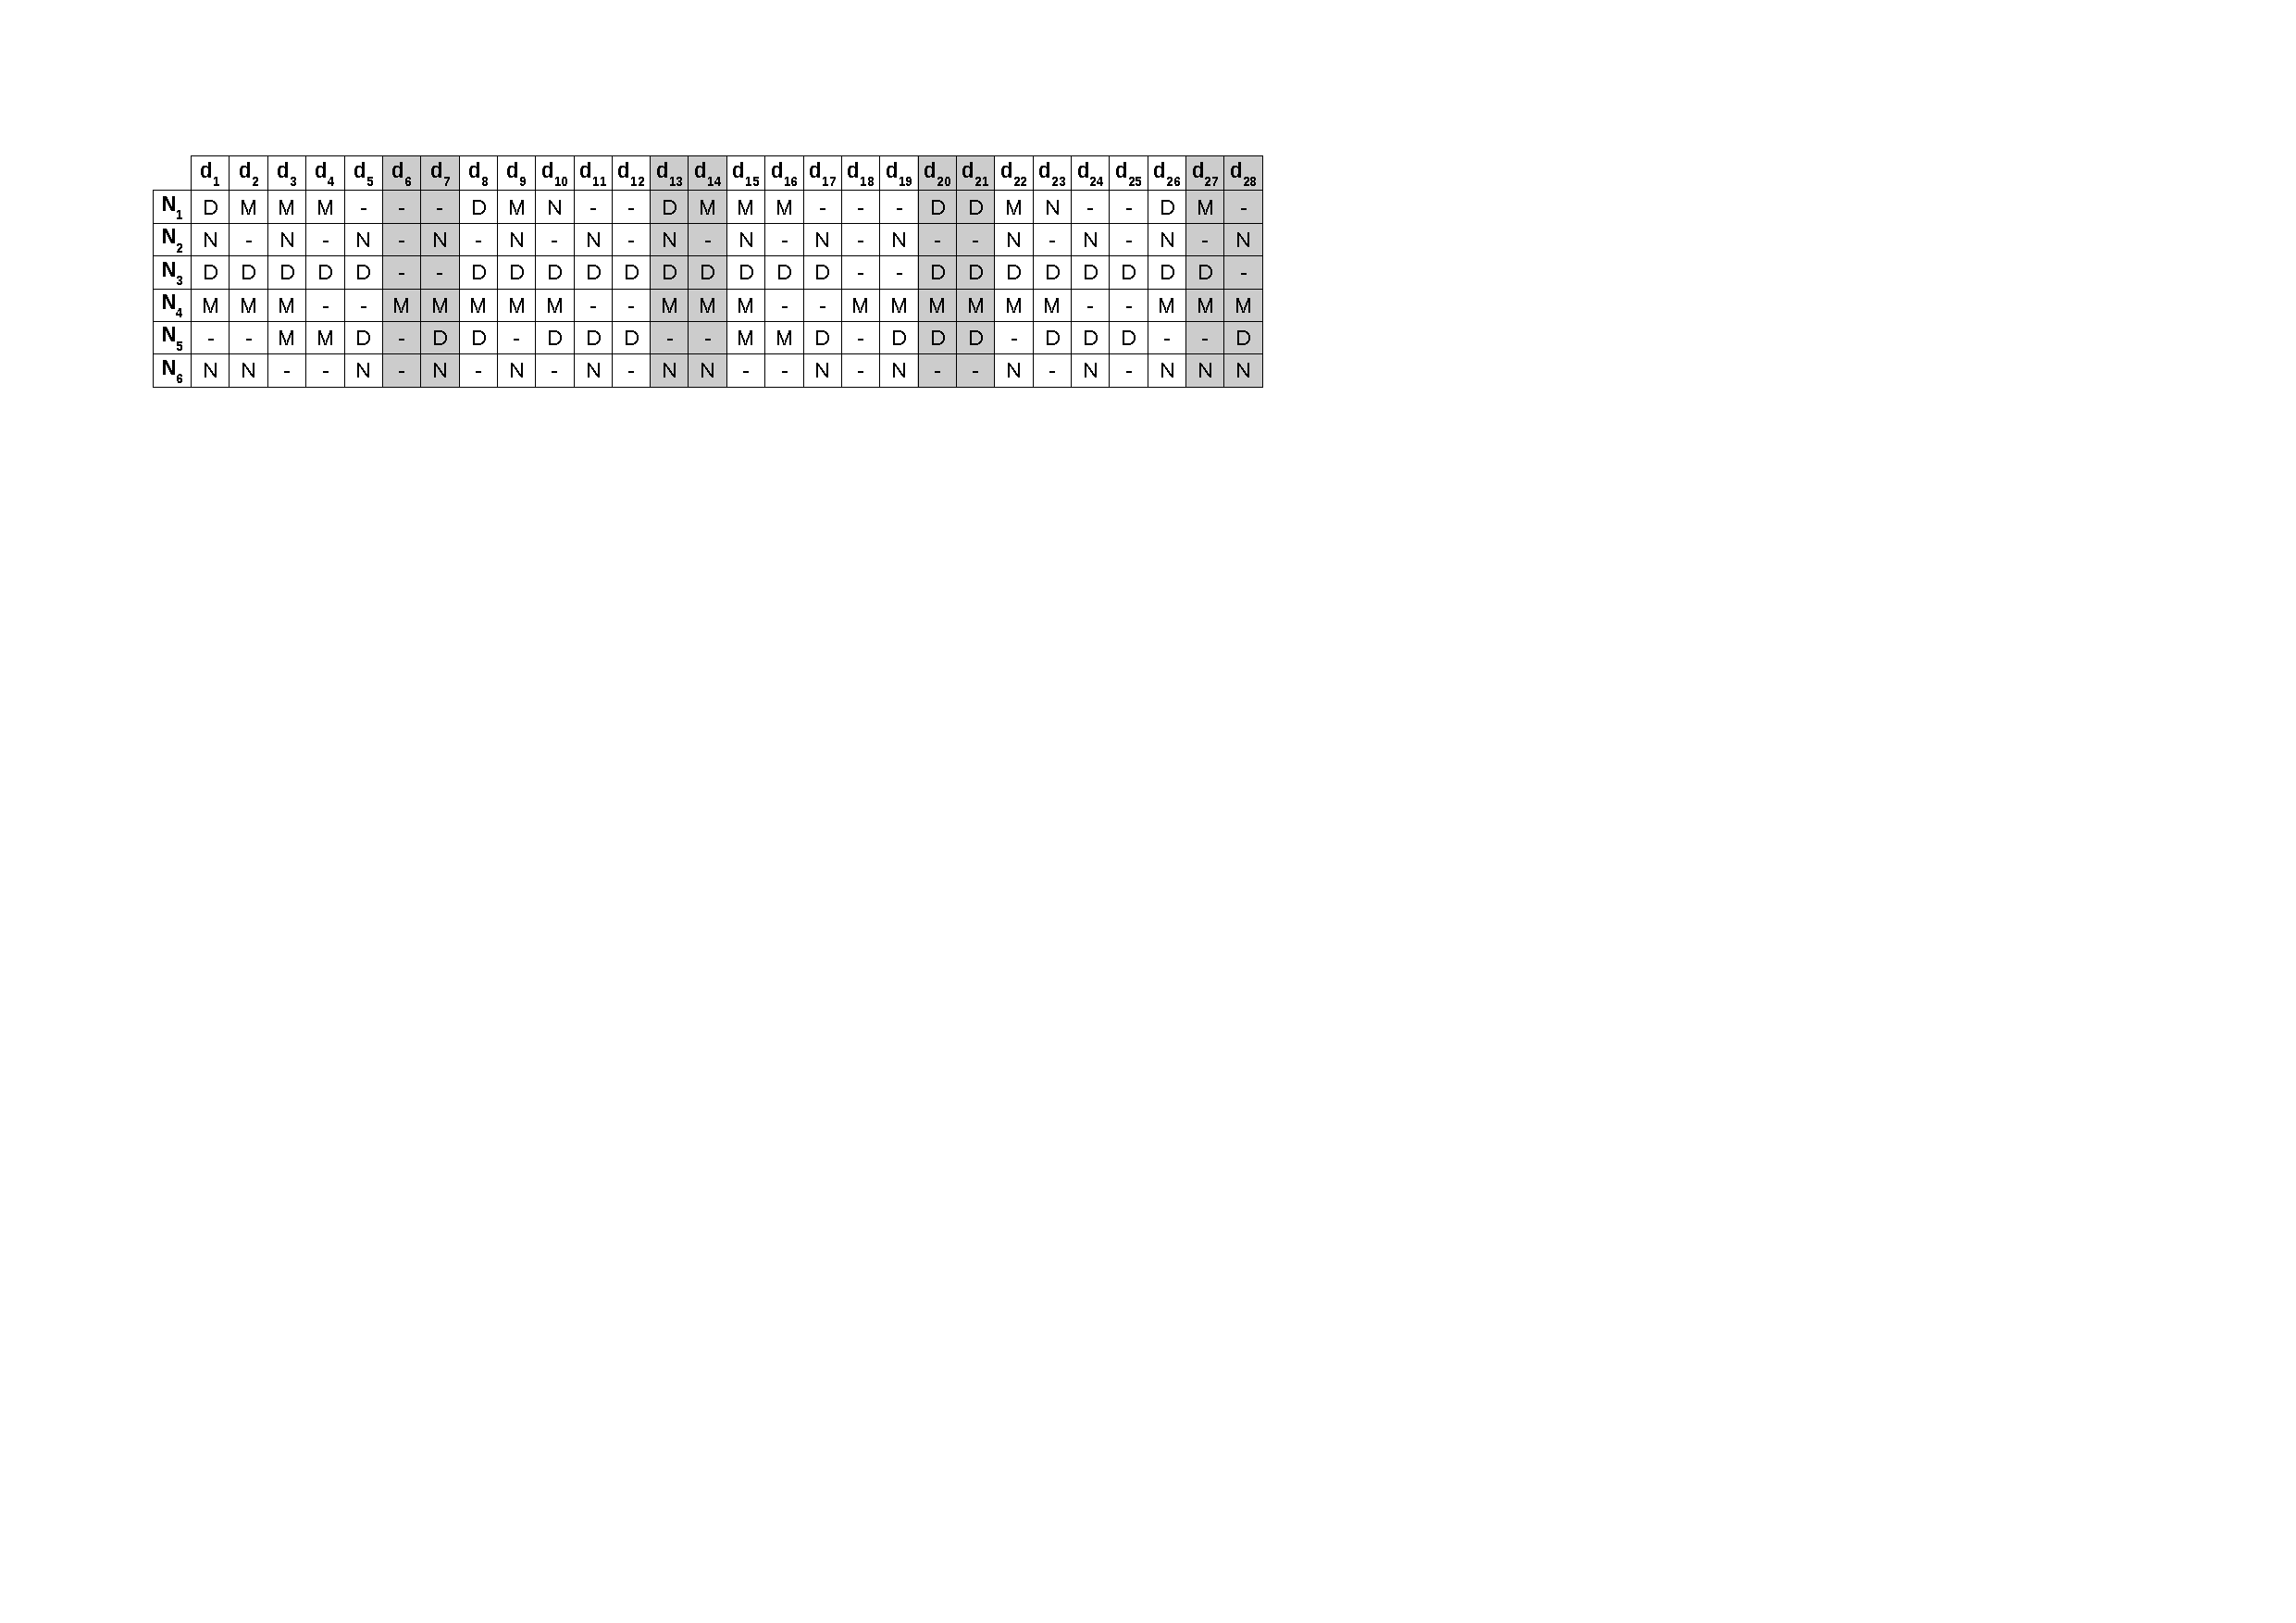
\includegraphics[width=15cm]{tabelaGeral.pdf}
\centering
\caption{Exemplo de escala com 28 dias ($d_1$ a $d_{28}$), seis enfermeiros ($N_1$ e $N_6$), três tipos de turnos e folga. }
\legend{Fonte: Do Autor}
\label{fig:escalaExemplo1}
\end{figure}

Devido ao grande número de possibilidades levados em consideração, a elaboração manual de uma escala pode consumir várias horas ou até mesmo dias para ser concluída e ainda assim gerar um resultado de baixa qualidade \cite{dias03, juliani07}. A criação de uma escala é um processo  complexo que influencia diretamente a qualidade da assistência do serviço de enfermagem. Uma escala deficiente pode resultar em várias  consequências negativas tais como: (i)~sobrecarga de trabalho, (ii)~faltas sem justificativa, (iii)~adoecimentos, (iv)~conflitos internos entre membros da equipe \cite{costa00, keretzky09, souza11} e (v)~erros na assistência de enfermagem que, em última instância, coloca em risco a vida dos pacientes.

O Problema de Escalonamento de Enfermagem\footnote{Na literatura o termo \emph{enfermeiros} também é utilizado. Neste trabalho optamos utilizar \emph{enfermagem}, pois a escala não é restrita apenas aos enfermeiros, incluindo outros profissionais da área.} (PEE) ainda é um desafio de pesquisa, além de ser considerado um problema de otimização NP-Difícil \cite{osogami2000classification}, as variações de requisitos requerem o desenvolvimento de métodos de resolução mais específicos. Devido a sua importância prática e teórica, vários métodos e abordagens computacionais foram propostos. Uma versão deste problema foi recentemente formalizada e proposta para a \textit{Second International Nurse Rostering Competition} (INRC-II)~\cite{ceschia2015second}. Nessa competição foi proposta a resolução do problema multi-estágio, onde a escala deve ser resolvida a cada semana considerando o histórico das semanas anteriores. Os requisitos da competição atendem aos principais problemas que são encontrados na realidade, dessa forma, é possível que um método com bom desempenho na INRC-II também possa ser aplicado com sucesso em situações reais. 

A primeira contribuição deste trabalho é o desenvolvimento de um método de resolução capaz de produzir boas soluções para a INRC-II e que tenha potencial para ser utilizado em cenários reais. Para isso, propomos um algoritmo baseado no \textit{Late Acceptance Hill Climbing} (LAHC) e sete diferentes movimentos para compor a vizinhança. O LAHC é uma metaheurística simples, com apenas um parâmetro, relativamente recente e pouco estudada na literatura. O algoritmo foi testado em comparação com outros competidores da INRC-II utilizando um extenso conjunto de instâncias. Os resultados obtidos demonstram que o método proposto é promissor, tem um bom desempenho e é relativamente mais simples que os dos demais concorrentes. A segunda contribuição é a proposição de um modelo de programação não linear inteiro com uma descrição mais fácil de compreender que o apresentado na definição da INRC-II.

O trabalho está organizado como segue. No Capítulo~\ref{ChapReview} uma revisão de literatura é apresentada considerando os principais
métodos utilizados para resolver o PEE, assim como a metaheurística usada 
neste trabalho. No Capítulo~\ref{ChapDef} o problema proposto pela INRC-II é detalhado. O algoritmo proposto é descrito no 
Capítulo~\ref{ChapLAHC}. No Capítulo~\ref{ChapR} serão apresentados os experimentos computacionais e a análise dos resultados. 
As considerações finais e trabalhos futuros são abordados no Capítulo~\ref{ChapConc}.


%------------------------------- CAPITULO --------------------------------------------------------------------------------------------
\chapter{Revisão de Literatura} \label{ChapReview}

Este capítulo apresenta uma visão geral sobre os trabalhos relacionados ao PEE e, em seguida, descreve o funcionamento da metaheurística que compõe o método proposto neste trabalho. Desta forma, o capítulo é dividido em duas seções. 
Na Seção \ref{SecMetodos} são discutidos os principais métodos propostos na literatura para resolução do PEE, com ênfase especial naqueles aplicados em competições internacionais. Na Seção \ref{Seclahc}, a metaheurística \emph{Late Acceptance Hill Climbing} é apresentada juntamente com um pseudocódigo e detalhes de implementação. 

\section{Trabalhos Relacionados} \label{SecMetodos}

O escalonamento de equipes de enfermagem faz parte de uma classe de problemas bastante ampla denomida Escalonamento de Pessoas. Problemas nesta classe vêm sendo estudados há décadas e inúmeras abordagens diferentes têm sido propostas para resolvê-los.
O trabalho de revisão mais recente nessa classe contabiliza uma lista de 291 publicações e as classifica de acordo com os métodos de solução e áreas de aplicação. Desta lista, 64 publicações são aplicações na área de escalonamemento de equipes de enfermagem \cite{van2013personnel}. 
Uma revisão bibliográfica mais específica do problema de escalonamento de enfermagem pode ser encontrada em \citet{burke2004state}. 
Nela, os autores comparam um grande número de publicações de acordo com vários critérios, incluindo propriedades do problema, variações na definição e métodos de resolução empregados.

No últimos anos, abordagens do tipo \emph{Matheuristic}, que combinam heurísticas com programação matemática, têm sido propostas com bastante frequência. Um exemplo é o trabalho do \citet{burke2010hybrid}, onde os autores utilizam Programação Inteira para encontrar uma solução inicial factível que, posteriormente, é melhorada com uma heurística \textit{Variable Neighborhood Search} (VNS). 
Técnicas mais sofisticados que também fazem o uso de programação matemática também são utilizadas como, por exemplo, o uso de Geração de
Colunas em \citet{mason1998nested}.

Devido ao grande número de variações existentes no PEE, a comparação de diferentes técnicas de resolução se tornou um dos principais desafios enfrentados pelos pesquisadores da área. 
Uma das primeiras iniciativas propostas para superar essa dificuldade foi a divulgação de um repositório de instâncias de teste, desenvolvido por pesquisadores da Universidade de Ghent, na Bélgica \cite{vanhoucke2007nsplib}. Esse repositório, conhecido como NSPLib, possibilitou a comparação entre as diferentes técnicas desenvolvidas para o problema a partir da criação de um \textit{website} onde as instâncias podem ser acessadas e as melhores soluções reportadas.

Outra iniciativa importante foi a realização de duas edições da \textit{International Nurse Rostering Competition}, referenciadas abreviadamente como INRC-I e INRC-II. Essas competições possibitaram que diferentes grupos de pesquisa resolvessem um problema bem definido utilizando um grupo de instâncias em comum.
Ambas as competições são detalhadas nas subseções seguintes, com foco especial para a segunda edição, cujo problema é objeto de estudo deste trabalho.

\subsection{INRC-I}

Nesta edição da competição foi proposta a resolução do PEE em uma única etapa, ou seja, sem subdividir o problema em semanas. O horizonte de planejamento foi de quatro semanas.
Os competidores foram avaliados em três conjuntos de instâncias que se diferem por tamanho e tempo de execução \cite{haspeslagh2010first}.
A seguir, são apresentadas as principais técnicas reportadas na literatura que obteram bons resultados ao serem aplicadas no problema da INRC-I.

O método vencedor da INRC-I proposto por \citet{valouxis2012systematic}, particionou cada instância em subproblemas e os resolveu sequencialmente utilizando programação matemática. Uma estratégia de duas fases foi implementada.
Na primeira fase é alocado o número de dias de trabalho para cada enfermeiro e dia da semana.
Na segunda fase são alocados turnos específicos para cada enfermeiro e dia.
Além disso, foram aplicadas técnicas de busca local para testar diferentes combinações de enfermeiros. 
Com esse método os autores ficaram em primeiro lugar em todos os conjuntos de instâncias.

\citet{burke10} abordaram o problema da INRC-I com dois algoritmos.
O primeiro algoritmo, um método baseado no \textit{ejection chain} foi aplicado em instâncias pequenas, onde o tempo para resolução do problema era de apenas 10 segundos. O segundo algoritmo, um método \textit{branch-and-price}, foi aplicado nas instância médias e grandes, onde o tempo para o processamento era de 10 e 600 minutos, respectivamente. 
O segundo algoritmo mostrou que em geral foi capaz de resolver muitas instâncias com otimalidade dentro do tempo estabelecido pela competição. 
%TODO ver a colocacao desse algoritmo
Este algoritmo ficou em segundo lugar nas instâncias médias e grandes.

No trabalho de \citet{bilgin2010hyper} foi proposta uma hiper-heurística distribuída em duas fases. 
Na primeira é selecionado um método heurístico aleatoriamente e um critério de aceitação baseado no \textit{Simulated Annnealing}.
Na segunda fase, uma versão extendida da heurística \textit{greedy shuffle} foi aplicada nas melhores soluções obtidas pela hiper-heurística.
%TODO ver se esse algoritmo é da competição pq n podia usar cplex
%Adicionalmente, os autores forneceram resultados computacionais para programação linear inteira usando IBM CPLEX.
Este algoritmo ficou em terceiro lugar na competição para as instâncias grandes e em quinto nas pequenas e médias.

%TODO qual a colocação geral do nonobe
\citet{nonobe2010inrc2010} utilizou uma metaheurística baseada no algoritmo \textit{constraint optimization problem} que implementa uma Busca Tabu para resolver o problema da INRC-I. O algoritmo ficou em segundo, terceiro e quarto lugar nas instâncias pequenas, médias e grandes, respectivamente. 
Mais informações sobre os métodos podem ser encontrados no site da competição\footnote{\url{https://www.kuleuven-kulak.be/nrpcompetition/competitor-ranking}}.

\subsection{INRC-II}

Em contraste com a primeira edição, a INRC-II apresenta um problema multi-estágios, onde soluções para as semanas individuais têm que ser produzidas sequencialmente, sem a informação sobre os requisitos das semanas posteriores.
A seguir serão apresentados os principais trabalhos relacionados ao problema da INRC-II. 

Uma vez que os métodos de resolução dos competidores que participaram da INRC-II não foram publicados em detalhes, pois apenas uma breve descrição está publicamente disponível, serão apresentadas outras publicações ocorridas após a competição.

O vencedor da INRC-II formulou o problema através de programação inteira mista baseada em fluxo de rede \textit{multi-commodity} \cite{romer2015multi}. 
Já o terceiro lugar na competição propôs um método de solução que usa hiper-heurística como base, analisando e produzindo sequências de heurísticas durante o processo de otimização \cite{kheirisequence}.
O quinto classificado na competição, a empresa ORTEC, uma companhia com sede na Holanda, propôs adicionar restrições fracas no algoritmo comercial da empresa para conseguir conectar as soluções das semanas e obter melhores resultados \cite{ortec}.

Os próximos trabalhos que serão listados abaixo desenvolveram novos métodos que não fizeram parte da competição. 
Cabe ressaltar que nesta avaliação, os autores não utilizaram as mesmas regras da INRC-II.

\citet{dang2016solving} implementou dois métodos para resolver o problema da \mbox{INRC-II}, um baseado em programação inteira mista e outro em \textit{Simulated Annealing}. O primeiro é um método exato que fez uso do IBM CPLEX, já o segundo envolveu uma composição de vizinhanças. Segundo os autores, os resultados preliminares mostram que os métodos implementados apresentaram resultados semelhantes aos dos finalistas.

\citet{mischek2016integer} propuseram um modelo matemático inteiro para a INRC-II que fez uso do IBM CPLEX, e mostrou que a adição de restrições a fim de possibilitar uma melhor análise das informações incompletas é necessária para alcançar resultados competitivos.
Também foi desenvolvida uma busca local baseada em uma combinação de \textit{Min-conflict} e Busca Tabu. 
Os autores reportaram que na maioria dos casos foi encontrada uma solução próxima da ótima. 


O trabalho mais recente, abordado por \citet{gomes2017variable}, apresenta um Geração de Colunas combinada com VNS para obter resoluções mais rapidamente, além de propor a heurística \textit{relax-and-fix} para obter soluções factíveis. O algoritmo melhorou em pelo menos 10\% os melhores resultados conhecidos para 29 intâncias \textit{hidden}, embora tenha utilizado um tempo muito superior ao da competição com execuções em paralelo e não tenha resolvido o problema por semanas.


\section{\textit{Late Acceptance Hill Climbing}}\label{Seclahc}

O \textit{Late Acceptance Hill Climbing} é um método estocástico iterativo utilizado para resolver problemas de otimização combinatória.
O método foi proposto por \citet{burke2008late} como uma metodologia de busca em trajetória simples e eficiente.
Durante o seu desenvolvimento foram considerados três objetivos principais para atender à proposta:
(i) não utilizar mecanismos artificiais de resfriamento como, por exemplo, o utilizado no \textit{Simulated Annealing}; 
(ii) utilizar de maneira eficiente informações de iterações anteriores da busca por meio de uma lista, de maneira similar ao mecanismo utilizado na Busca Tabu;
(iii) utilizar um critério de aceitação tão simples quanto o do \textit{Hill Climbing}.

Assim como no \textit{Simulated Annealing}, o LAHC começa a busca com uma solução inicial aleatória que é modificada por um procedimento iterativo com o objetivo de minimizar ou maximizar uma função de custo $C(.)$.
A cada iteração uma solução candidata~$s'$ é gerada a partir da solução atual~$s$. 
Essa solução~$s'$ pode ser aceita como a nova solução~$s$, ou seja, $s = s'$, se atender ao seguinte critério de aceitação: $C(s') <= C(s)$ ou $C(s')$ é menor do que o custo que a solução $s$ tinha a $t$ iterações atrás. 
Para viabilizar esse critério, o algoritmo mantém uma lista com os custos das soluções $s$ das últimas $t$ iterações. 

O funcionamento da lista ocorre de forma que a cada solução aceita o seu custo é inserido no início da lista e o último elemento é descartado. Para que a complexidade dessas operações seja constante, a lista é representada em um formato circular. 
Para isso, a implementação de acesso aos índices da lista ocorre com os operadores de módulo, como podemos ver na linha 9 do algoritmo, onde $v$ é o índice da lista calculado como iteração $i$ módulo do tamanho da lista $t$.

A Figura~\ref{alg:lahc} apresenta o pseudocódigo do algoritmo LAHC descrito em \citet{burke2012late}.  
O método \texttt{LAHC} recebe como parâmetro de entrada um tamanho~$t$ da lista.
Na Linha 1, uma solução inicial $s$ é gerada e as posições da lista $L_w$, onde $w \in {1... t}$,  são inicializadas com $C(s)$ (linha 4). Na Linha 8, a cada iteração $i$, uma solução candidata $s'$ é gerada e avaliada pelo critério de aceitação.
Uma solução candidata é aceita se for igual ou melhor que o custo $L_v$ da lista, ou igual ou melhor que o custo da solução corrente ($C(s') \le C(s)$) (linha 10).
Quando $s'$ é aceita, $s$ é atualizada com $s'$ (linha 11). 
A atualização da melhor solução $s^*$ encontrada é realizada apenas caso $C(s) <= C(s^*)$ (linha 12). Em caso afirmativo, a nova solução incumbente é guardada (linha 13). 
Note que $s$ é igual a $s'$ em caso de aceitação apenas, mas em caso de rejeição a solução não é atualizada.
Nas linhas 16 e 17 a lista é atualizada com a solução corrente e o número de iterações é incrementado. O laço recomeça até que a condição de parada seja satisfeita.

\begin{figure}[ht!]
\iniciaproc{LAHC}{$t$}
      \STATE Gera solução inicial $s$ 
      \STATE $s* \gets s$
      \FOR {$w \in {0... t-1}$}
        \STATE $L_w \gets C(s)$
      \ENDFOR
      \STATE $i \gets 0$
      \REPEAT 
         \STATE Gera uma solução candidata $s'$ 
         \STATE $v \gets i$ mod $t$
         \IF {$C(s') \le L_v$ $ou$ $C(s') \le C(s)$}
            \STATE $s \gets s'$

            \IF {$C(s) < C(s^*)$}
                \STATE $s^* \gets s$
            \ENDIF
         \ENDIF
         \STATE $L_v \gets C(s)$
         \STATE $i \gets i + 1$
      \UNTIL{condição de parada seja satisfeita}
      \RETURN $s^*$

\fimproc{alg:lahc}{Pseudo-code of the LAHC algorithm}
\vspace{-2mm}
\caption{Pseudo-código da LAHC proposta.}
\label{alg:lahc}
\end{figure}



%------------------------------- CAPITULO --------------------------------------------------------------------------------------------

\chapter{Definição do Problema} \label{ChapDef}

Neste capítulo será descrito em detalhes o Problema de Escalonamento de Enfermagem (PEE) definido na INRC-II.
Primeiramente, uma visão geral do PEE é apresentada na Seção \ref{sec:visaogeral}. Em seguida, as restrições consideradas no problema são classificadas e enumeradas na Seção \ref{sec:restricoes}.
E finalmente, na Seção \ref{sec:modelo}, o PEE é definido formalmente através da proposição de dois modelos matemáticos. Todos os conceitos e definições introduzidos a seguir serão referenciados ao longo dos próximos capítulos.

\section{Visão Geral do PEE}\label{sec:visaogeral}

O objetivo do problema é construir uma escala para um conjunto de enfermeiros, considerando um horizonte de planejamento que geralmente varia de uma a oito semanas.
Cada dia da escala é subdividido em um conjunto de turnos pré-estabelecidos como, por exemplo, \textit{day} (D), \textit{late} (L) e \textit{night} (N)\footnote{Optamos por não traduzir os nomes dos cargos e turnos adotados no problema da INRC-II visto que eles nem sempre possuem uma correspondência adequada utilizada no Brasil.\label{f1}}. Desta forma, o processo de alocação de cada enfermeiro consiste em designar para cada dia da escala, o turno em que ele irá trabalhar e qual qualificação irá exercer. 
Cada enfermeiro possui um determinado conjunto de qualificações como, por exemplo, $Nurse$, $HeadNurse$ ou $CareTaker$\textsuperscript{\ref{f1}}. Em cada alocação, um enfermeiro pode exercer apenas uma de suas qualificações e pode estar alocado no máximo em um turno de trabalho por dia.


A Figura~\ref{fig:escalaExemplo} apresenta uma escala simplificada do PEE composta por sete dias ($d_1$ a $d_7$) e dois enfermeiros ($N_1$ e $N_2$).
Em cada célula é apresentada a alocação de um enfermeiro em um turno e a qualificação que está sendo exercida. Observe que, enquanto o enfermeiro $N_1$ está alocado no turno $N$ no dia $d_1$ com a qualificação $HeadNurse$, no dia $d_3$ ele está de folga, indicada pelo símbolo ``-''.

\begin{figure}[H]
\includegraphics[width=12cm]{tabelaEnf.pdf}
\centering
\caption{Escala com sete dias ($d_1$ a $d_7$), dois enfermeiros ($N_1$ e $N_2$), três turnos ($N$=\textit{Night}, $E$=\textit{Early} 
e $D$=\textit{Day}) e folgas representadas por ``-''.}
\legend{Fonte: Do Autor}
\label{fig:escalaExemplo}
\end{figure}

Além de construir a escala, ainda é necessário minimizar as violações das restrições, como por exemplo, o número máximo de dias trabalhados, o número mínimo de folgas, entre outras que serão apresentadas em mais detalhes na Seção~\ref{sec:restricoes}.

Os problemas de escalonamento de enfermeiros geralmente são resolvidos considerando todo o horizonte de planejamento em uma única vez. Porém, na INRC-II, o horizonte de planejamento é dividido em múltiplos estágios onde cada estágio precisa ser resolvido separadamente. Na INRC-II, cada estágio corresponde ao período de uma semana. 

\begin{comment}
Para que os parâmetros de cada semana sejam estabelecidos e as semanas anteriores possam ser consideradas na solução, essas informações são armazenadas em três diferentes arquivos de dados:

\begin{itemize}
	\item Dados do cenário: válido para todo o horizonte de planejamento, contém informações gerais sobre turnos, qualificações, enfermeiros e contratos.
	\item Dados da semana: válido apenas para o estágio atual, neste arquivo estão as preferências individuais de cada enfermeiros e os valores da cobertura.
	\item Dados do histórico: contém informações relevantes sobre atribuições do fim da semana anterior, como número de dias consecutivos trabalhados, último turno trabalhado, número de dias de folga, etc.
\end{itemize}
\end{comment}

Ao construir uma escala para um estágio é necessário conhecer informações da escala do estágio anterior para considerar algumas restrições do problema. Chamamos estas informações de dados de \emph{borda}. Estas informações situam-se em uma estrutura de dados denominada \emph{histórico}, que também inclui outros dados cumulativos dos estágio anteriores. 
A cada estágio resolvido é gerado uma histórico que será utilizado para resolução do estágio posterior. 
Este modo de resolução é denominado \emph{multi-estágio}. 

No PEE existem várias restrições que precisam ser calculadas utilizando informações do histórico, como por exemplo, a restrição que limita o número de dias consecutivos trabalhados. Para avaliar essa restrição, deve-se considerar os dias trabalhados no final do estágio anterior e o início do estágio atual. A Figura \ref{fig:escalaSeq} ilustra um exemplo desta restrição em que um enfermeiro pode trabalhar no máximo 3 dias consecutivos. Se cada estágio for avaliado individualmente, esta restrição não teria violação. No entanto, considerando a continuidade na conexão dos estágios, pode-se perceber que o enfermeiro $N_1$ está excedendo em 1 dia o limite máximo da restrição.  

\begin{figure}[H]
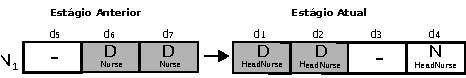
\includegraphics[width=12cm]{exsequencia.pdf}
\centering
\caption{Escala apresentando um exemplo de conexão do estágio atual com as informações do histórico (estágio anterior).}
\label{fig:escalaSeq}
\legend{Fonte: Do Autor}
\end{figure}


Uma das principais dificuldades desse tipo de problema é que para avaliar a escala do estágio atual é necessário considerar os resultados das semanas anteriores e desenvolver mecanismos para estimar como a resolução do estágio atual irá interferir na resolução dos posteriores. Na Figura \ref{fig:escalaMultiestagio} é apresentado um exemplo da resolução multi-estágio com um horizonte de planejamento composto por quatro semanas. O fluxo de resolução segue uma ordem em que, por exemplo, a solução da semana 2 apenas pode ser avaliada após a escala da semana 1 ser construída, o mesmo ocorre com as semanas seguintes. A Figura~\ref{fig:escalaf} apresenta a solução final do problema que é composta pela conexão das soluções de cada estágio da Figura~\ref{fig:escalaMultiestagio}.

\begin{figure}[ht!]
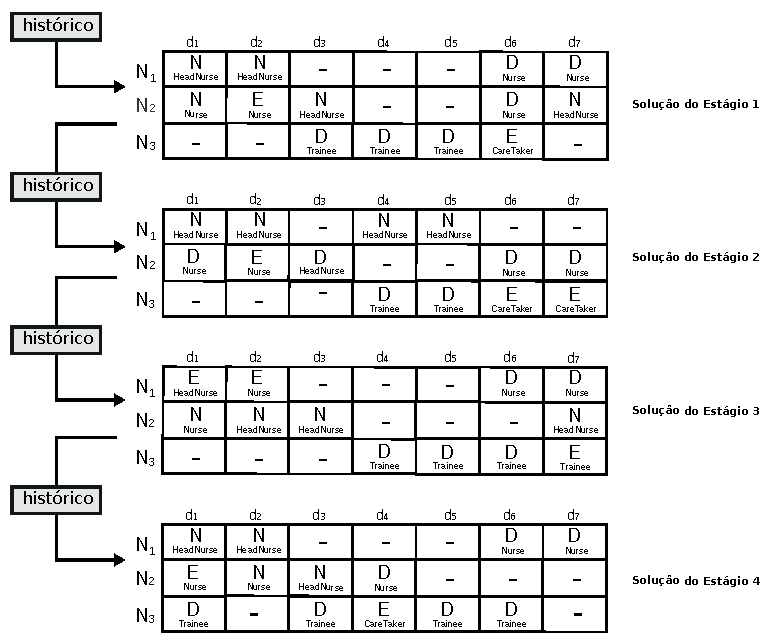
\includegraphics[width=12cm]{escalageral.pdf}
\centering
\caption{Exemplo de escala multi-estágio para um planejamento de quatro semanas e três enfermeiros.}
\label{fig:escalaMultiestagio}
\legend{Fonte: Do Autor}
\end{figure}

\begin{figure}[ht!]
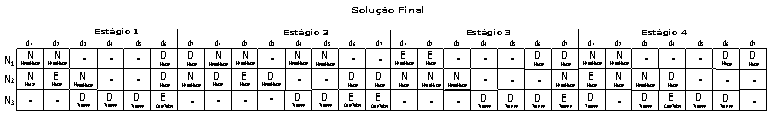
\includegraphics[width=16cm]{estagiof.pdf}
\centering
\caption{Exemplo de escala final composta por 4 estágios e três enfermeiros.}
\label{fig:escalaf}
\legend{Fonte: Do Autor}
\end{figure}


\newpage

\section{Tipos de Restrições} \label{sec:restricoes}

De acordo com a especificação da INRC-II, o PEE considera dois tipos de restrições: \emph{restrições fortes} e \emph{restrições fracas}. As restrições fortes devem ser obrigatoriamente satisfeitas para que uma escala possa ser utilizada na prática. Já as restrições fracas, caso sejam violadas geram uma escala de pior qualidade. Para cada violação de uma restrição fraca existe um peso para a penalização na função objetivo.
Se ao menos uma restrição forte for violada, a solução é considerada \emph{infactível}. Ambos os tipos de restrições são apresentados a seguir: 

\bigskip
\noindent\textbf{Restrições Fortes:}
\begin{itemize}
    \item [\textbf{H1}:] O enfermeiro deve trabalhar apenas um turno por dia.
    \item [\textbf{H2}:] Para cada dia e turno, existe um número mínimo de enfermeiros que devem ser alocados em cada qualificação. Esse requisito é chamado de \textit{cobertura mínima}.
    \item [\textbf{H3}:] A sucessão de turnos deve ser válida. Por exemplo, enfermeiro que trabalha no turno da noite não pode no dia seguinte trabalhar no turno da manhã.
    \item [\textbf{H4}:] Ao atribuir uma determinada qualificação para um enfermeiro, esta deve pertencer necessariamente ao conjunto de qualificações do enfermeiro.
\end{itemize}

\bigskip
\noindent\textbf{Restrições Fracas:}
\begin{itemize}
    \item [\textbf{S1}:] Para cada dia e turno, existe um número ótimo de enfermeiros que devem ser alocados em cada qualificação. Esse requisito é chamado de \textit{cobertura ótima}. Para cada enfermeiro faltando para atingir a cobertura ótima incide um dado custo. Enquanto os excedentes não são penalizados.

    \item [\textbf{S2}:] Esta restrição estabelece limites para alocações consecutivas descritos a seguir:
       \begin{itemize}[nosep]
			\item [\textbf{a})] Número mínimo de dias consecutivos trabalhados.
			\item [\textbf{b})] Número máximo de dias consecutivos trabalhados.
			\item [\textbf{c})] Número mínimo de alocações consecutivas no mesmo turno.
			\item [\textbf{d})] Número máximo de alocações consecutivas no mesmo turno.			
		\end{itemize}  

    \item [\textbf{S3}:] Esta restrição estabelece limites para dias de folga consecutivos, descritos a seguir:
		\begin{itemize}[nosep]
			\item [\textbf{a})] Número mínimo de dias consecutivos de folga.
			\item [\textbf{b})] Número máximo de dias consecutivos de folga.	
		\end{itemize}  
		
    \item [\textbf{S4}:] Esta restrição estabelece as seguintes preferências para os enfermeiros:
		\begin{itemize}[nosep]
			\item [\textbf{a})] Enfermeiro prefere não trabalhar em um determinado turno.
			\item [\textbf{b})] Enfermeiro prefere não trabalhar em um determinado dia.
		\end{itemize} 
    \item [\textbf{S5}:] Esta restrição estabelece que, caso o enfermeiro tenha preferência por fins de semana completo, então ele deve trabalhar sábado e domingo ou em nenhum desses dias.
    \item [\textbf{S6}:] Esta restrição estabelece os seguintes limites considerando todos os estágios:
		\begin{itemize}[nosep]
			\item [\textbf{a})] Número máximo de dias trabalhados.
			\item [\textbf{b})] Número mínimo de dias trabalhados.
		\end{itemize} 

    \item [\textbf{S7}:] Número máximo de fins de semana trabalhados. 
\end{itemize}

Enquanto a maioria das restrições podem ser calculadas adequadamente no contexto de um estágio, as restrições S6 e S7 precisam de informações de todos os estágios. Desta forma, podemos classificar as restrições conforme o escopo. As restrições S6 e S7 são \emph{restrições globais} e as demais são \emph{restrições locais}.

\section{Modelagem Matemática} \label{sec:modelo}

Nesta seção é proposta uma modelagem utilizando programação inteira não linear para o problema da INRC-II considerando todos as restrições fortes e fracas descritas na Seção~\ref{sec:restricoes}. 
Esta modelagem é baseada na formulação matemática disponibilizada pela INRC-II em \cite{ceschia2015model}. Como o problema tem muitas restrições, esse modelo tem como objetivo principal descrever de uma forma mais clara o PEE. 
Além disso, a modelagem apresentada permite compreender o PEE tanto do ponto de vista global (multi-estágio), quanto do ponto de vista local (único estágio). 

Para isso propomos dois modelos $\mu_1$ e $\mu_2$. O primeiro trata apenas as restrições locais de um estágio, enquanto o segundo inclui restrições globais e considera todos os estágios. 
Os modelos $\mu_1$ e $\mu_2$ são apresentados, respectivamente, nas Seções \ref{umestagio} e \ref{multiestagio}. A notação matemática usada nas formulações é apresentada nas Tabelas \ref{tab:conjuntos}, \ref{tab:parametros} e \ref{tab:variaveis}.

\begin{table}[H]
\centering
\caption{Notação dos conjuntos utilizados na formulação matemática.}
\small
\begin{tabularx}{\linewidth}{l@{}X}
\hline\noalign{\smallskip}
\textbf{Conjuntos}{~~~~~~~~~~}  & Definição  \\
\noalign{\smallskip}\hline\noalign{\smallskip}
	$e \in E$  & conjunto de estágios. \\
	$n \in N$  & conjunto de enfermeiros. \\
	$d \in D$  & conjunto de dias. \\
	$w \in W$  & conjunto de dias do fim de semana ($w \subseteq D$). \\
	$s \in S$  & conjunto de turnos. \\
	$s \in S'$  & conjunto de turnos, exceto o turno da folga. \\
	$k \in K$  & conjunto de qualificações. \\
	$(s_1, s_2) \in F$  & conjunto de sucessões proibidas, onde o turno $s_2$ não pode vir após $s_1$. \\ 
	$K_n$  & conjunto de qualificações do enfermeiro $n$ ($K_n \subseteq K$). \\
	$P_{nds} \in \{0,1\}$ & assume 1 se o enfermeiro $n$ prefere não ser alocado no turno $s$ do dia $d$. \\
	$P_{nd} \in \{0,1\}$ &  assume 1 se o enfermeiro não quer ser alocado em nenhum turno do dia $d$, ou seja, ele quer folga no dia $d$.\\
	$(u,v) \in B$ & conjunto de tuplas $(u,v)$ tal que $u \in D, v \in D$ onde $u \leq v$. Cada par representa um possível bloco de alocações consecutivas em um estágio.  \\
	$(i,j) \in B_{uv}$ & conjunto de blocos $(i,j)$ que são incompatíveis com o bloco $(u,v)$. Ou seja, $(i,j) \in B$, $(u,v) \in B$: $i \leq u, v \leq j$, $(i,j) \neq (u,v)$.\\
\noalign{\smallskip}\hline
\end{tabularx}
\label{tab:conjuntos}
\end{table}

\newpage
%------------------------------------------------------------------------------------------------------------------------------
%\noalign{\medskip}
\begin{table}[H]
\centering
\caption{Notação dos parâmetros utilizados na formulação matemática.}
\small
\begin{tabularx}{\linewidth}{l@{}X}
\hline\noalign{\smallskip}
\textbf{Parâmetros}{~~~~~}  & Definição  \\
\noalign{\smallskip}\hline\noalign{\smallskip}
 $V^-_{dsk} \in \mathbb{N^*}$   & número mínimo de enfermeiros com qualificação $k$ requerida no dia $d$ e turno $s$ (cobertura mínima).  \\
 $V^*_{dsk} \in \mathbb{N^*}$   & número ótimo de enfermeiros com qualificação $k$ requerida no dia $d$ e turno $s$ (cobertura ótima).  \\
 $W^{S1}, ..., W^{S7}$ & peso das restrições S1 a S7.\\
$L^+_{n} \in \mathbb{N^*}$   & número máximo de dias consecutivos trabalhados para o enfermeiro $n$.\\
$L^-_{n} \in \mathbb{N^*}$   & número mínimo de dias consecutivos trabalhados para o enfermeiro $n$.\\
$L^+_{ns} \in \mathbb{N^*}$   & número máximo de alocações consecutivas do turno $n$ para o enfermeiro $n$.\\
$L^-_{ns} \in \mathbb{N^*}$   & número máximo de alocações consecutivas do turno $n$ para o enfermeiro $n$.\\
$G^+_{n} \in \mathbb{N^*}$   & número máximo de folgas consecutivas para o enfermeiro $n$.\\
$G^-_{n} \in \mathbb{N^*}$   & número mínimo de folgas consecutivas para o enfermeiro $n$.\\
$V_{n} \in \{0,1\}$   & assume 1 se o enfermeiro $n$ precisa trabalhar todo o fim de semana.\\
$h^{e}_{n} \in \mathbb{N^*}$ & número de dias consecutivos trabalhados no fim do estágio $e-1$. Ou seja, $h^{e}_{n} = \max_{i \in D} \left(b^{e-1}_{ni|D|} * (|D|-i+1)\right).$\\
$h^{e}_{ns} \in \mathbb{N^*}$ & número de alocações consecutivas no turno $s$ no fim do estágio $e-1$. Ou seja, $h^{e}_{ns} = \max_{i \in D} \left(b^{e-1}_{ni|D|s} * (|D|-i+1)\right).$\\
$\delta^{e} \in \mathbb{N^*}$ & custo das alocações consecutivas no final do estágio $e-1$.  Ou seja: \\
						& $\delta^{e} = \sum_{n \in N} \sum_{i \in D} \left(^{(e-1)}C^{S2a}_{ni|D|} + ^{(e-1)}C^{S2b}_{ni|D|}\right) + $\\ 
						& ~~~~~~~~~~$ \sum_{n \in N} \sum_{i \in D} \sum_{s \in S'}\left(^{(e-1)}C^{S2c}_{ni|D|s} + ^{(e-1)}C^{S2d}_{ni|D|s}\right) + $ \\
						& ~~~~~~~~~~$ \sum_{n \in N} \sum_{i \in D} \left(^{(e-1)}C^{S3a}_{ni|D||S|} + ^{(e-1)}C^{S3b}_{ni|D||S|} \right)$ \\
$Q^+_{n} \in \mathbb{N^*}$   & número máximo de dias trabalhados considerando todos os estágio para o enfermeiro $n$.\\
$Q^-_{n} \in \mathbb{N^*}$   & número mínimo de dias trabalhados considerando todos os estágio para o enfermeiro $n$.\\
$R^+_{n} \in \mathbb{N^*}$   & número máximo de fins de semana trabalhados.\\

\noalign{\smallskip}\hline
\end{tabularx}
\label{tab:parametros}
\end{table}



\begin{table}[H]
\centering
\caption{Notação das variáveis utilizadas na formulação matemática.}
\small
\begin{tabularx}{\linewidth}{l@{}X}
\hline\noalign{\smallskip}
\textbf{Variáveis}{~~~~~~~~~~~~}  & Definição  \\
\noalign{\smallskip}\hline\noalign{\smallskip}
$x^e_{ndsk} \in \{0,1\}$        & Assume 1 quando o enfermeiro $n$ está alocado no dia $d$ no turno $s$ com a qualificação $k$ no estágio $e$.  \\
$C^{S1}_{dsk} \in \mathbb{N^*}$   & número de enfermeiros faltando no turno $s$ do dia $d$ para atingir a cobertura ótima definida por $C^*_{dsk}$.  \\
$b^e_{nij} \in  \{0,1\} $ & Assume 1 quando o enfermeiro $n$ começa um bloco de alocações consecutivas iniciando no dia $i$ e terminando no dia $j$ no estágio $e$.\\
$b^e_{nijs} \in  \{0,1\} $ & Assume 1 quando o enfermeiro $n$ começa um bloco de alocações consecutivas com o turno $s$ iniciando no dia $i$ e terminando no dia $j$ no estágio $e$.\\
$^eC^{S2a}_{nij} \in \mathbb{N^*}$   & número de dias excedendo o limite $L^+_{n}$ no bloco de trabalho $(i,j) \in B$ para um enfermeiro $n$ no estágio $e$.  \\
$^eC^{S2b}_{nij} \in \mathbb{N^*}$   & número de dias faltando para atingir o limite $L^-_{n}$ no bloco de trabalho $(i,j) \in B$ para um enfermeiro $n$ no estágio $e$.  \\
$^eC^{S2c}_{nijs} \in \mathbb{N^*}$   & número de dias excedendo o limite $L^+_{ns}$ no bloco de trabalho $(i,j) \in B$ para um enfermeiro $n$ considerando apenas o turno $s$ no estágio $e$.  \\
$^eC^{S2d}_{nijs} \in \mathbb{N^*}$   & número de dias faltando para atingir o limite $L^-_{ns}$ no bloco de trabalho $(i,j) \in B$ para um enfermeiro $n$ considerando apenas o turno $s$ no estágio $e$.  \\
$^eC^{S3a}_{nij} \in \mathbb{N^*}$   & número de dias de folga excedendo o limite $G^+_{n}$ no bloco de trabalho $(i,j) \in B$ para um enfermeiro $n$ no estágio $e$.  \\
$^eC^{S3b}_{nij} \in \mathbb{N^*}$   & número de dias de folga faltando para atingir o limite $G^-_{n}$ no bloco de trabalho $(i,j) \in B$ para um enfermeiro $n$ no estágio $e$.  \\
$C^{S6a}_{n} \in \mathbb{N^*}$   & número de dias de trabalho excedendo o limite $Q^+_{n}$ para um enfermeiro $n$ em todos os estágios. \\
$C^{S6b}_{n} \in \mathbb{N^*}$   & número de dias de trabalho faltando para atingir o limite $Q^-_{n}$ para um enfermeiro $n$ em todos os estágios. \\
$C^{S7}_{n} \in \mathbb{N^*}$   & número de fins de semana trabalhados excedendo o limite $R^+_{n}$ para um enfermeiro $n$ para todos os estágios. \\
\noalign{\smallskip}\hline
\end{tabularx}
\label{tab:variaveis}
\end{table}

%--------------------------- SECAO MODELO DE UM ESTAGIO --------------------------------------------------------
\subsection{Modelo de um estágio ($\mu_1$)}\label{umestagio}

O modelo apresentado a seguir pode ser utilizado para resolver um único estágio $e \in E$ considerando apenas as restrições locais.

%------------------------------------------------------------------------------------------------------------------------------
\begin{samepage}
\begin{align}
   \textbf{min~~} Z_e =~~&W^{S1} \sum_{d \in D}\sum_{s \in S}\sum_{k \in K} C^{S1}_{dsk}    + \\
  					&W^{S2ab}  \sum_{n \in N}\sum_{(i,j) \in B} (C^{S2a}_{nij} + C^{S2b}_{nij}) + \\
  					& W^{S2cd}  \sum_{n \in N}\sum_{(i,j) \in B}\sum_{s \in S'} (C^{S2c}_{nijs} + C^{S2d}_{nijs}) + \\
					& W^{S3}    \sum_{n \in N}\sum_{(i,j) \in B} (C^{S3a}_{nij} + C^{S3b}_{nij}) + \\
					& W^{S4}    \sum_{n \in N}\sum_{d \in D}\sum_{s \in S'}\sum_{k \in K} (x^e_{ndsk} * P_{nds} + x^e_{ndsk} * P_{nd}) + \label{eS4}\\
					& W^{S5}    \sum_{n \in N} V_{n} * ( 1- \prod_{d \in W} \sum_{s \in S'}\sum_{k \in K} x^e_{ndsk}) -\delta^e  \label{eS5} 
\end{align}  

\begin{align}
& \sum_{s \in S} \sum_{k \in K} x^e_{ndsk} = 1    && \forall n \in N, d \in D \label{eH1} \\
& \sum_{n \in N} x^e_{ndsk} \geq V^-_{dsk}   && \forall d \in D, s \in S, k \in K \label{eH2} \\
& \sum_{k \in K} (x^e_{n,d-1,s_1,k} + x^e_{n,d,s_2,k}) \leq 1 && _{\forall n \in N, d \in D\setminus \{1\}, (s_1,s_2) \in F} \label{eH3a} \\
& \sum_{k \in K} (x^{e-1}_{n,d,s_1,k} + x^e_{n,1,s_2,k}) \leq 1 && _{\forall n \in N, d = |D|, (s_1,s_2) \in F} \label{eH3b} \\
& x^e_{ndsk} = 0   && _{\forall n \in N, d \in D, s \in S, k \in K\setminus K_n} \label{eH4} \\
& C^{S1}_{dsk} = \max\{ V^*_{dsk} - \sum_{n \in N} x^e_{ndsk}, 0\} && \forall d \in D, s \in S', k \in K \label{eS1} \\
& b^e_{nuv} \texttt{=} \max \{0, \hspace{-1mm}\sum_{u \leq d \leq v} \sum_{s \in S'} \sum_{k \in K} x^e_{ndsk} \texttt{-} (v \texttt{-}u) \texttt{-}\hspace{-1mm} \sum_{(i,j) \in B_{uv}}\hspace{-1mm} b^e_{nij}\} && \forall n \in N, (u,v) \in B \label{eS2aux1} \\
& b^e_{nuvs} \texttt{=} \max \{0, \sum_{u \leq d \leq v} \sum_{k \in K} x^e_{ndsk} \texttt{-} (v \texttt{-}u) \texttt{-} \hspace{-1mm}\sum_{(i,j) \in B_{uv}} \hspace{-1mm} b^e_{nijs}\} && \forall n \in N, (u,v) \in B, s \in S \label{eS2aux2} \\
& ^eC^{S2a}_{nij} \texttt{=}  \max\{0, b^e_{nij} * ((j - i +1 + h^e_{n}*\lfloor 1/i \rfloor) - L^+_{n})\} && \forall n \in N, (i,j) \in B \label{eS2a} \\
& ^eC^{S2b}_{nij} \texttt{=}  \max\{0, b^e_{nij} * (L^-_{n} - (j - i +1  + h^e_{n}*\lfloor 1/i \rfloor))\} && \forall n \in N, (i,j) \in B \label{eS2b} \\
& ^eC^{S2c}_{nijs} \texttt{=}  \max\{0, b^e_{nijs} * ((j - i +1  + h^e_{ns}*\lfloor 1/i \rfloor) - L^+_{ns})\} && \forall n \in N, (i,j) \in B, s \in S'\label{eS2c} \\
& ^eC^{S2d}_{nijs} \texttt{=}  \max\{0, b^e_{nijs} * (L^-_{ns} - (j - i +1 + h^e_{ns}*\lfloor 1/i \rfloor))\} && \forall n \in N, (i,j) \in B, s \in S' \label{eS2d} \\
& ^eC^{S3a}_{nij} \texttt{=}  \max\{0, b^e_{nijs} * ((j - i +1  + h^e_{ns}*\lfloor 1/i \rfloor) - G^+_{n})\} && \forall n \in N, (i,j) \in B, s \texttt{=} |S|\label{eS3a} \\
& ^eC^{S3b}_{nij} \texttt{=}  \max\{0, b^e_{nijs} * (G^-_{n} - (j - i +1  + h^e_{ns}*\lfloor 1/i \rfloor))\} && \forall n \in N, (i,j) \in B, s \texttt{=} |S| \label{eS3b} \\
& x^e_{ndsk} \in \{0,1\}  &&  \forall n \in N, d \in D, s \in S, k \in K  \notag  \\
& b^e_{nijs},  b^e_{nij} \in \{0,1\}  &&  \forall n \in N, (i,j) \in B, s \in S \notag \\
& ^eC^{S2a}_{nij}, ^eC^{S2b}_{nij}, ^eC^{S2c}_{nijs}, ^eC^{S2d}_{nijs}, ^eC^{S3a}_{nij}, ^eC^{S3b}_{nij} \in \mathbb{N^*} && \forall n \in N, (i,j) \in B, s \in S \notag 
\end{align}
\end{samepage}
%------------------------------------------------------------------------------------------------------------------------------

A função objetivo $Z_e$ calcula parcialmente o valor de uma solução do PEE pois considera apenas um estágio $e \in E$ e ignora as restrições globais S6 e S7. A função $Z_e$ é ponderada com pesos correspondentes às violações das restrições fracas S1, S2 (subdividida em dois: S2a com S2b, e S2c com S2d), S3, S4 e S5. Além disso, no final da função é subtraído o parâmetro $\delta^e$, que se refere ao custo das penalidades de restrições de consecutividade do estágio anterior ($e-1$) que, devido a conexão entre estágios também são contabilizados no estágio $e$.

O conjunto de restrições~(\ref{eH1}) modela a restrição forte H1 garantindo que exatamente um turno seja alocado em cada dia para cada enfermeiro.
O conjunto de restrições~(\ref{eH2}) modela a restrição forte H2 garantindo que a cobertura mínima definida por $V^-_{dsk}$ seja atendida.
Os conjuntos de restrições (\ref{eH3a}) e~(\ref{eH3b}) modelam a restrição forte H3 garantindo que duas alocações consecutivas não ocorram em sucessões proibidas. Particularmente, o conjunto de restrições~\ref{eH3b} é necessário para considerar a restrição H3 na conexão entre o estágio atual e o anterior.  
O conjunto de restrições~(\ref{eH4}) modela restrição forte H4 impedindo que um enfermeiro seja alocado nas qualificações que ele não possui.
O conjunto de restrições~(\ref{eS1}) modela restrição S1 contabilizando na variável $^eC^{S1}_{dsk}$ o número de enfermeiros faltando para atingir a cobertura ótima definida por $V^*_{dsk}$.
Os conjuntos de restrições~(\ref{eS2aux1}) e~(\ref{eS2aux2}) servem para auxiliar na identificação de blocos de alocações necessários para calcular as restrições fracas S2 e S3. Particularmente, o conjunto de restrições~(\ref{eS2aux1}) garante que a variável $b^e_{nuv}$ será ativada apenas quando o enfermeiro $n$ tiver um bloco de alocações consecutivas iniciando no dia $u$ e terminando no dia $v$. 
Analogamente, o conjunto de restrições~(\ref{eS2aux2}) garante que a variável $b^e_{nuvs}$ será ativada apenas quando o enfermeiro $n$ tiver um bloco de alocações consecutivas no turno $s$ iniciando no dia $u$ e terminando no dia $v$. Esta modelagem que identifica blocos de alocações consecutivas foi inspirada na abordagem apresentada no trabalho de \citet{dorneles2012impact}.
Os conjuntos de restrições~(\ref{eS2b}) e~(\ref{eS2a}) modelam, respectivamente, as restrições fracas S2a e S2b, contabilizando nas variáveis $^eC^{S2a}_{nij}$ e $^eC^{S2b}_{nij}$ o número de dias faltando/excedendo o limite mínimo/máximo de dias consecutivos trabalhados.
Observe que a expressão $\lfloor 1/i \rfloor$ serve para considerar a parcela $h^e_{ns}$ apenas quando $i=1$. Esta situação especial ($i=1$) é necessária para conectar as alocações consecutivas do final do estágio anterior com blocos de alocações que se iniciam no dia 1 do estágio atual.
Analogamente, os conjuntos de restrições~(\ref{eS2c}),~(\ref{eS2d}),~(\ref{eS3a}) e~(\ref{eS3b}) modelam a restrição fracas S2c, S2d, S3a e S3b contabilizando nas variáveis $^eC^{S2c}_{nijs}$, $^eC^{S2d}_{nijs}$, $^eC^{S3a}_{nij}$ e $^eC^{S3b}_{nij}$ o número de alocações faltando/excedendo o limite mínimo/máximo de alocações consecutivas.
S4 e S5 são modeladas diretamente na função objetivo, respectivamente nas equações~(\ref{eS4}) e~(\ref{eS5}).

\subsection{Modelo multi-estágio ($\mu_2$)}\label{multiestagio}

No modelo multi-estágio são consideradas todas as restrições do PEE, incluindo as restrições globais S6 e S7. O modelo é apresentado abaixo:

\begin{align}
   \textbf{min~~}  &Y =  \sum_{e \in E} Z_e + \sum_{n \in N} (W^{S6} C^{S6a}_n + W^{S6} C^{S6b}_n + W^{S7} C^{S7}_n) 
\end{align}                     
\begin{align}
& C^{S6a}_n =  \max\{0, \sum{e \in E}\sum_{d \in D} \sum_{s \in S'}\sum_{k \in K} x^e_{ndsk} - Q^+_{n}\} && \forall n \in N \label{eS6a}\\
& C^{S6b}_n =  \max\{0, Q^-_{n} - \sum{e \in E}\sum_{d \in D} \sum_{s \in S'}\sum_{k \in K} x^e_{ndsk}\} && \forall n \in N \label{eS6b}\\
& C^{S7}_n =  \max\{0,\sum_{e \in E}\max_{d \in W, k \in K, s \in S'} (x^e_{ndsk}) - R^+_{n}\}  && \forall n \in N \label{eS7} \\
& C^{S6a}_{n}, C^{S6b}_{n}, C^{S7}_{n} \in \mathbb{N^*} && \forall n \in N \notag
\end{align}

A função objetivo $Y$, além de minimizar a função $Z_e$, para todos os estágios $e \in E$ do modelo $\mu_1$, inclui nas parcelas seguintes a contabilização das violações das restrições S6a, S6b e S7 ponderadas com os pesos $W^{S6}$ e $W^{S7}$.

O conjunto de restrições (\ref{eS6a}) e (\ref{eS6b}) modelam as restrições fracas S6a e S6b contabilizando nas variáveis $C^{S6a}_n$ e $C^{S6b}_n$ o número de dias excedendo/faltando o limite máximo/minimo de dias trabalhados em todos os estágios. 
O conjunto de restrições (\ref{eS7}) modela a restrição fraca S7 contabilizando na variável $C^{S7}_n$ o número de fins de semana que excedem o limite máximo de fins de semana trabalhados em todos os estágios. 

Podemos destacar que o modelo $\mu_2$ é capaz de encontrar a solução ótima do PEE caso todos os estágios possam ser resolvidos ao mesmo tempo de maneira exata. No entanto, mesmo que isso fosse permitido dentro das regras da competição, até o momento, não são conhecidos métodos de resolução eficientes para resolver o modelo $\mu_2$.

%------------------------------- CAPITULO --------------------------------------------------------------------------------------------
\chapter{Algoritmo Proposto} \label{ChapLAHC}

Neste trabalho propomos abordar o PEE definido no Capítulo \ref{ChapDef}. 
O método proposto é baseado na metaheurística LAHC cujo algortimo genérico é apresentado na Seção~\ref{Seclahc}.
Esse capítulo foca nos detalhes de implementação desse algoritmo que são específicos para aplicação do método no problema estudado. 
O capítulo é organizado como segue. Na Seção~\ref{SecEstruturaSol} é apresentada a estrutura de dados da solução.
Na Seção~\ref{SecGeracaoSol} é apresentada a forma como a solução inicial é gerada. 
Na Seção~\ref{SecCalcSemanal} é apresentada a função objetivo utilizada, incluindo um cálculo para a estimativa dos custo globais em cada estágio. 
Finalmente, a Seção \ref{SecVizinhança} especifica o modo como a solução candidata será obtida a partir de uma estrutura de vizinhança.


\section{Estrutura de Dados da Solução}\label{SecEstruturaSol}

Para representar uma solução é preciso definir uma estrutura para armazenar as alocações de cada enfermeiro para cada dia da semana.
Uma alocação é composta por um turno e uma qualificação. Para isso foi utilizada uma matriz $A_{m \times n}$, onde $m$ é o total de enfermeiros e $n$ o número de dias da semana. Cada posição da matriz armazena o par \emph{(turno, qualificação)}. Dessa forma, a estrutura obriga que apenas um turno seja atribuído ao enfermeiro em cada dia, garantindo que a restrição H1 seja sempre satisfeita.
Além da matriz $A$, junto da solução são armazenados vários índices para permitir um cálculo eficiente da função objetivo.

\section{Geração da Solução Inicial}\label{SecGeracaoSol}

Conforme indicado na Linha 1 do pseudocódigo da Figura \ref{alg:lahc}, o LAHC requer uma solução inicial aleatória para iniciar o processo de melhoria.
A construção desta solução é realizada para cada enfermeiro, preenchendo todas as suas alocações semanais com um turno e uma qualificação aleatória.
Para garantir que a restrição H4 nunca seja violada, a qualificação do enfermeiro é selecionada apenas entre aquelas que ele possui. 


\section{Função Objetivo}\label{SecCalcSemanal}

O cálculo da função objetivo para problemas multi-estágio tem como principal desafio a avaliação da solução quando existem restrições globais, as quais requerem informações de todos os estágios. Isso ocorre no problema da INRC-II para as restrições S6 e S7.
Esse tipo de problema onde a demanda futura é incerta foi abordado por \citet{romer2016future} no contexto da INRC-II. Neste trabalho, os autores avaliaram o impacto que essas restrições causam na solução caso sejam consideradas apenas no final de todos os estágios. Após aplicar diferentes estratégias, os resultados computacionais mostraram que até o mais simples cálculo de previsão determinístico conseguiu melhorar consideravelmente as soluções. 
Desta forma, propomos a seguir algumas funções para estimar as restrições S6 e S7. Na implementação do LAHC, essas estimativas são utilizadas em conjunto com a função $Z_e$ para compor a função objetivo do algoritmo proposto.

\subsection{Estimativa da Restrição S6}\label{subs6}

Relembrando o que foi visto no Capítulo \ref{ChapDef}, a restrição S6 estabelece um número máximo ($Q^+_{n}$) e um número mínimo ($Q^-_{n}$) de dias trabalhados para todos os estágios. Com o objetivo de obter novos limites dessa restrição para cada estágio $e$ e enfermeiro $n$ são realizados cálculos apresentados e discutidos abaixo.

Para que seja possível estabelecer uma distribuição igualitária do número máximo e mínimo de dias trabalhados para os estágios que ainda não foram resolvidos, é preciso considerar o número de dias trabalhados nos estágios anteriores $\beta(n,e)$ para cada enfermeiro $n$. A Equação (\ref{hw}) contabiliza os dias trabalhados de todos os estágios anteriores ao estágio $e$. Caso o estágio atual seja o primeiro ($e=0$), então $\beta(n,0)=0$.  

\begin{align}
& \beta(n,e) = \sum_{i=0}^{i=e-1}\sum_{d \in D} \sum_{s \in S'}\sum_{k \in K} x^i_{ndsk}   \label{hw} 
\end{align}

Nas Equações (\ref{ests6a}) e (\ref{ests6b}) são calculados os novos limites para o número máximo~$Q^{+}(n,e)$ e mínimo~$Q^{-}(n,e)$ de dias trabalhados para cada enfermeiro $n$ e estágio $e$.
Por exemplo, na Equação \ref{ests6a}, se um enfermeiro possui $Q^{+}_n=20$, $\beta(n,1)=5$ e $e=1$, ou seja, o enfermeiro $n$ trabalhou 5 dias no estágio 0, então ele ainda possui no máximo 15 dias para trabalhar em todos os estágios. A fim de estimar esses dias restantes de forma igualitária para todos os estágios, dividimos esse valor pelos estágios que ainda restam ser escalonados.
Por exemplo, seja uma escala onde $|E=4|$, ainda faltariam 3 estágios para serem resolvidos. Logo, o novo valor limite $Q^{+}(n,1)=5$, pois $15/3$=5 no estágio 1.

\begin{align}
& Q^{+}(n,e) = \max\{0, \lceil (( Q^+_{n} - \beta(n,e)) / (|E|-e) + 0.5)\rceil\} \label{ests6a}\\
& Q^{-}(n,e) = \lfloor ( Q^-_{n} - \beta(n,e)) / (|E|-e) \rfloor   \label{ests6b} 
\end{align}

Nas Equações (\ref{cs6a}) e (\ref{cs6b}) são apresentadas a contabilização de dias trabalhados excedentes ou faltantes, respectivamente. 
Estes valores são calculados por $C^{S6a}(n,e)$ e $C^{S6b}(n,e)$, os quais são penalizados na função objetivo.

\begin{align}
& C^{S6a}(n,e) = max\{0, \sum_{d \in D} \sum_{s \in S'}\sum_{k \in K} x^e_{ndsk} -  Q^{+}(n,e)\} \label{cs6a}\\
& C^{S6b}(n,e) = max\{0,  Q^{-}(n,e) - \sum_{d \in D} \sum_{s \in S'}\sum_{k \in K} x^e_{ndsk}\} \label{cs6b} 
\end{align}

\subsection{Estimativa da Restrição S7}\label{subs7}

Relembrando o que foi visto no Capítulo \ref{ChapDef}, a restrição S7 estabelece um número máximo $R^+_{n}$ de fins de semana trabalhados para todos os estágios. De maneira semelhante aos cálculos de estimativa da restrição S6, visto na Seção \ref{subs6}, a restrição S7 também precisa obter novos limites para cada estágio $e$ e enfermeiro $n$. Os cálculos realizados são apresentados e discutidos abaixo.

Primeiramente, consideramos o número de fins de semana trabalhados nos estágios anteriores $\gamma(n,e)$ para cada enfermeiro $n$. Na Equação (\ref{hds7})  contabiliza os dias trabalhados de todos os estágios anteriores ao estágio $e$. Caso o estágio atual seja o primeiro ($e=0$), então $\gamma(n,0)=0$.  

\vspace{-0.8cm}

\begin{align}
& \gamma(n,e) = \sum_{i=0}^{i=e-1} \min\{1, \sum_{d \in W} \sum_{s \in S'}\sum_{k \in K}x^i_{ndsk}\}  \label{hds7} 
\end{align}

Da mesma forma que o cálculo da restrição S6, a Equação (\ref{rs7}) determina um novo limite para o número máximo $R^{+}(n,e)$ de fins de semana trabalhados para cada enfermeiro $n$ e estágio $e$. 

\begin{align}
&R^{+}(n,e) = \max\{0, \lceil (( R^+_{n} - \gamma(n,e)) / (|E|-e) +0.5)\rceil\}  \label{rs7}
\end{align}

Na Equação (\ref{cs7}) apresenta a contabilização de fins de semana trabalhados excedentes a qual é penalizada na função objetivo através da variável $C^{S7}(n,e)$.

\begin{align}
& C^{S7}(n,e) = max\{0, \sum_{d \in D} \sum_{s \in S'}\sum_{k \in K} x^e_{ndsk} -  R^{+}(n,e)\}  \label{cs7}
\end{align}


\section{Geração da Solução Candidata} \label{SecVizinhança}

No LAHC uma nova solução candidata $s'$ é gerada em cada iteração, conforme procedimento indicado na Linha 8 do pseudocódigo da Figura \ref{alg:lahc}.
No método proposto, a solução $s'$ é escolhida aleatoriamente a partir de uma estrutura de vizinhança $\mathcal{N}(s)$, onde $s$ é a solução atual, dessa forma, $s' \in \mathcal{N}(s)$.
A estrutura $\mathcal{N}(s)$ adota um esquema semelhante ao de \citet{fonseca2016late} em que diversos tipos de movimentos são utilizados para compor a vizinhança. 
Neste trabalho em específico propomos sete tipos de movimentos $M_1$ a $M_7$ que serão detalhados nas subseções seguintes.

\subsection{Modificação de turno ($M_1$)}
Este movimento consiste em alterar aleatoriamente o turno em que um enfermeiro está alocado em um dado dia.
A Figura \ref{fig:vizinhanca1} apresenta um exemplo de aplicação desse movimento na solução $s$, gerando a solução $s'$. 

\begin{figure}[ht!]
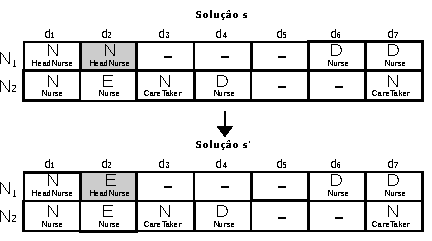
\includegraphics[width=12cm]{v1.pdf}
\centering
\caption{Exemplo do movimento $M_1$ em que o enfermeiro $N_1$ no dia $d_2$ tem seu turno alterado de $N$ na solução $s$ para $E$ na solução $s'$.}
\label{fig:vizinhanca1}
\legend{Fonte: Do Autor}
\end{figure}

\subsection{Troca de turnos em bloco ($M_2$)}
Este movimento consiste em trocar um bloco de alocações de turno entre dois enfermeiros. 
Um bloco é uma sequência de turnos consecutivos com tamanho limitado a 7.  
Tanto o tamanho do bloco quanto o dia de início do bloco são escolhidos aleatoriamente.
A Figura \ref{fig:vizinhanca2} apresenta um exemplo de aplicação desse movimento na solução $s$, gerando a solução $s'$. 

\begin{figure}[ht!]
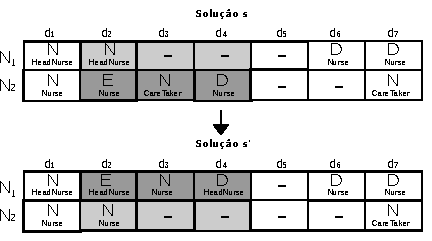
\includegraphics[width=12cm]{v2.pdf}
\centering
\caption{Exemplo do movimento $M_2$ em que as alocações de turno do enfermeiro $N_1$ são trocadas com as do $N_2$ considerando um bloco 
de tamanho 3 que inicia no dia $d_2$.} 
\label{fig:vizinhanca2}
\legend{Fonte: Do Autor}
\end{figure}

\subsection{Modificação de qualificação ($M_3$)}

Este movimento consiste em alterar aleatoriamente uma qualificação em que um enfermeiro está alocado em um dado dia.
A qualificação do enfermeiro é selecionada apenas entre aquelas que ele possui. Entre todos os movimentos, este é o único que modifica a alocação da qualificação. A Figura \ref{fig:vizinhanca3} apresenta um exemplo de aplicação desse movimento na solução $s$, gerando a solução $s'$. 


\begin{figure}[ht!]
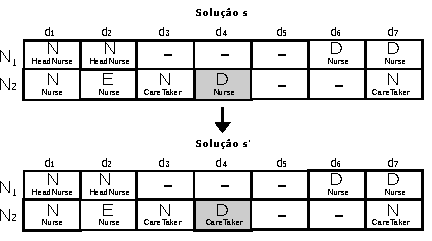
\includegraphics[width=12cm]{v3.pdf}
\centering
\caption{Exemplo do movimento $M_3$ em que o enfermeiro $N_2$ no dia $d_4$ tem sua quaificação alterada de $Nurse$ na solução $s$ para $CareTaker$ na solução $s'$.}
\label{fig:vizinhanca3}
\legend{Fonte: Do Autor}
\end{figure}

\subsection{Atribuição de uma folga ($M_4$)}
Este movimento consiste em selecionar um enfermeiro aleatório que esteja trabalhando em um dado dia e atribuir a ele um turno de folga.
A Figura \ref{fig:vizinhanca4} apresenta um exemplo de aplicação desse movimento na solução $s$, gerando a solução $s'$. 

\begin{figure}[ht!]
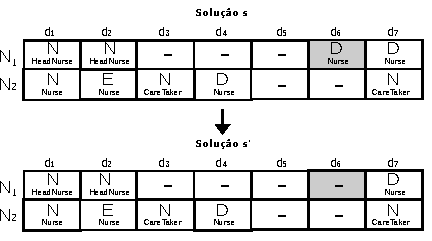
\includegraphics[width=12cm]{v4.pdf}
\centering
\caption{Exemplo do movimento $M_4$ em que o enfermeiro $N_1$ no dia $d_6$ tem seu turno alterado de $D$ na solução $s$ para um turno de folga na solução $s'$.} 
\label{fig:vizinhanca4}
\legend{Fonte: Do Autor}
\end{figure}

\subsection{Fim de semana completo ($M_5$)}
Este movimento consiste em alterar as alocações dos turnos do fim de semana (dias $d_6$ e $d_7$) de um enfermeiro, considerando os seguintes casos para os dias $d_6$ e $d_7$:

\begin{enumerate}
	\item Se ambos estiverem alocados os turnos de trabalhos, então atribui-se um turno de folga para ambos.
	\item Se ambos estiverem de folga, então atribui-se turnos aleatório de trabalho para~\mbox{ambos}. 
	\item Se apenas um dos dias estiver alocado com uma folga, então procede-se com 50\% de chance de executar o caso 1 ou o caso 2. 
\end{enumerate} 
Observe que este movimento visa facilitar as restrições S5 e S7. 
A Figura \ref{fig:vizinhanca5} apresenta um exemplo de aplicação desse movimento na solução $s$, gerando a solução $s'$. 

\begin{figure}[ht!]
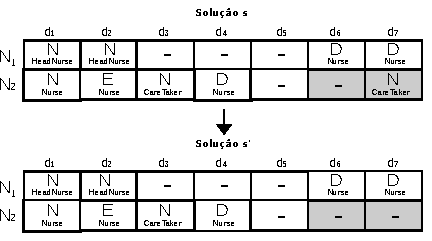
\includegraphics[width=12cm]{v5.pdf}
\centering
\caption{Exemplo do movimento $M_5$ executando o caso 3 para o enfermeiro $N_2$. Visto que na solução $s$ apenas o dia $d_6$ tinha uma folga, 
avaliou-se a chance de 50\% e, neste exemplo, resultou na execução do caso 1, atribuindo uma folga para o dia $d_7$ na solução~$s'$.} 
\label{fig:vizinhanca5}
\legend{Fonte: Do Autor}
\end{figure}

\subsection{Troca de turno de trabalho com turno de folga ($M_6$)}
Este movimento consiste em trocar as alocações dos turnos entre dois enfermeiros em um dado dia. Os enfermeiros são selecionados de forma 
que um deles deve estar alocado em um turno de folga e o outro alocado em um turno de trabalho.
A Figura \ref{fig:vizinhanca6} apresenta um exemplo de aplicação desse movimento na solução $s$, gerando a solução $s'$. 

\begin{figure}[ht!]
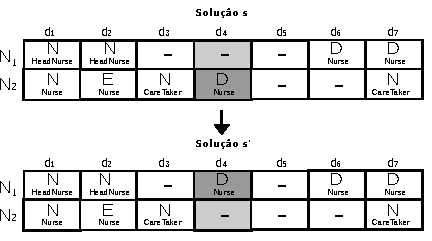
\includegraphics[width=12cm]{v6.pdf}
\centering
\caption{Exemplo do movimento $M_6$ em que o enfermeiro $N_1$ tem seu turno trocado com o enfermeiro $N_2$ no dia $d_4$.} 
\label{fig:vizinhanca6}
\legend{Fonte: Do Autor}
\end{figure}


\subsection{Troca de blocos para um enfermeiro ($M_7$)}
Este movimento inverte dois blocos de alocação de turno de um enfermeiro, atuando apenas nos dias~$d_1$ a~$d_5$.
Para realizar esse movimento, um ponto de corte $p$ é sorteado para definir os dois blocos que serão invertidos.
O primeiro bloco tem início no dia~$d_1$ e termina no dia~$p$, já o segundo bloco começa no dia~$p+1$ e termina no dia~$d_5$. 
Observe que, em especial, este movimento não modifica o número de violações das restrições S5, S6 e S7 além de manter parcialmente a satisfação das restrições H3, S2 e S3 dentro dos blocos. 
A Figura \ref{fig:vizinhanca7} apresenta um exemplo de aplicação desse movimento na solução~$s$, gerando a solução~$s'$. 

\begin{figure}[ht!]
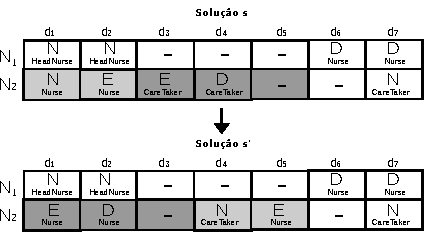
\includegraphics[width=12cm]{v7.pdf}
\centering
\caption{Exemplo do movimento $M_7$ com ponto de corte $p=2$ para o enfermeiro $N_2$.} 
\label{fig:vizinhanca7}
\legend{Fonte: Do Autor}
\end{figure}

\section{Seleção do Movimento}

Os movimentos da vizinhança são selecionados de acordo com uma probabilidade dada a cada movimento. A definição destes valores será detalhada na Seção~\ref{exp1}. Na Figura~\ref{fig:roleta}, é apresentado um exemplo hipotético de como poderia ser distribuída a probabilidade dos sete movimentos propostos nesse trabalho, de $M_1$ a $M_7$, de forma que a soma das probabilidades sempre resulte em~100\%. Percebe-se que, por exemplo, $M_3$ e $M_7$ possuem as maiores chances de serem selecionados, com~25\% cada. Já $M_4$ e $M_5$ têm as menores chances de serem selecionados, com~8\% cada.

\begin{figure}[ht!]
\includegraphics[width=6cm]{roleta.pdf}
\centering
\caption{Exemplo de distribuição de probabilidade dos movimentos $M_1$ a $M_7$.\\} 
\legend{Fonte: Do Autor}
\label{fig:roleta}
\end{figure}

%------------------------------- CAPITULO --------------------------------------------------------------------------------------------
\chapter{Experimentos Computacionais} \label{ChapR}

Neste capítulo serão apresentados experimentos computacionais para o algoritmo proposto neste trabalho. O objetivo dos experimentos é responder as seguintes questões: 
\medskip
\begin{enumerate}[nosep]
   \item[i)] Qual combinação de parâmetros é mais apropriada para o algoritmo proposto?
   \item[ii)] Como o algoritmo se compara com os demais competidores?
   \item[iii)] O método proposto conseguiria ser classificado para a final? 
   \item[iv)] O método proposto é robusto quanto à reprodução dos resultados?
\end{enumerate}
\medskip

O capítulo está estruturado da seguinte forma, na Seção \ref{instancia} são apresentadas as instâncias da competição, na Seção \ref{confParam} são detalhados as configurações do ambiente experimental e, finalmente, nas Seções \ref{exp1}-\ref{exp4} são apresentados diferentes experimentos com uma análise de resultados.

\section{Instâncias}\label{instancia}

Para avaliar o algoritmo proposto foram utilizados dois conjuntos de instâncias da INRC-II, \textit{late} e \textit{hidden}, disponibilizadas \textit{online}\footnote{\url{http://mobiz.vives.be/inrc2/?page_id=20}}. 
As instâncias \textit{late} são compostas por conjuntos de 30, 40, 50, 60, 80, 100 e 120 enfermeiros. Cada grupo de enfermeiros possui quatro instâncias, duas com um horizonte de planejamento de quatro semanas e as outras duas com oito semanas, totalizando assim 28 instâncias no conjunto \textit{late}.
Já as instâncias \textit{hidden} são compostas por conjuntos de 35, 70 e 110 enfermeiros. Cada grupo de enfermeiros possui vinte
instâncias, dez delas com horizonte de planejamento de quatro semanas e as outras dez com oito semanas, totalizando 60 instâncias no conjunto \textit{hidden}.

As instâncias são identificadas por nomes padronizados que as caracterizam em número de enfermeiros e horizonte de planejamento. Por exemplo, n030w4\_0\_1-7-1-8 é uma instância com 30 enfermeiros e 4 semanas, e n110w8\_0\_2-1-1-7-2-6-4-7 tem 110 enfermeiros e 8 semanas.

\section{Ambiente Experimental}\label{confParam}

Todos os experimentos realizados foram conduzidos em um servidor equipado com um processador \textit{Intel Xeon 2.83GHz, 8 GB de memória RAM} e um sistema operacional \textit{Linux Ubuntu 16.04.1 LTS} de 64 \textit{bits}. 
Para a implementação do algoritmo proposto foi utilizada a linguagem de programação~\textit{C++} e o compilador \textit{g++}\footnote{\url{https://gcc.gnu.org/}} (versão 5.4.0) usando as flags \textit{--std=c++11 -O3}. 
Para a computação do processo de variação de amostras foi usado \emph{Mersenne Twister}, um gerador de números randômicos \cite{mersenne}.
Todos os resultados dos experimentos foram certificados pelo validador disponibilizado pelos organizadores da INRC-II\footnote{\url{http://mobiz.vives.be/inrc2/?page_id=245}\label{site}} usando as mesmas regras competição.

Na INRC-II, o tempo limite para cada semana é determinado por uma ferramenta de \textit{benchmark} \textsuperscript{\ref{site}}. Dependendo do número de enfermeiros da instância e do poder de processamento do computador, o \textit{benchmarking} fornece um tempo limite distinto. Na Tabela~\ref{tab:instances}, a primeira linha apresenta diferentes número de enfermeiros, a segunda linha indica o tempo limite por semana, em segundos, correspondente para cada conjunto de enfermeiros.

\begin{table}[ht!]
\caption{Tempo limite por semana determinado pela ferramenta de \textit{benchmark} da INRC-II para instâncias de tamanhos variados.}
\medskip
\small
\label{tab:instances}
\centering
%\scalebox{0.8}{
\begin{tabular}{r|rrrrrrrrrr}
\textit{Enfermeiros} & 30 & 35 & 40 & 50 & 60 & 70 & 80 & 100 & 110 & 120 \\
\hline
\textit{Tempo(s)} &  59.7 & 82.0 & 104.5 & 149.3 & 194.1 & 238.5 & 283.7 & 373.3 & 417.4 & 462.0    \\
\end{tabular}
\end{table}

Na INRC-II participaram 15 equipes de competidores, listados na Tabela \ref{tab:competidores}. Na primeira coluna os competidores são identificados por um \emph{id} seguido pelo nome da equipe e informações na segunda e terceira coluna, respectivamente. Os campos das informações que contém ``-'', significa que não foram encontradas informações sobre a respectiva equipe.
A INRC-II teve a participação de competidores de diversos países com equipes de alto nível de pesquisadores especializados em resolver problemas de otimização combinatória. 
Duas dessas equipes são brasileiras, a \emph{GOAL} da Universidade Federal de Ouro Preto e a \emph{INF\_UFRGS} da Universidade Federal do Rio Grande do Sul. Também podemos destacar as equipes \emph{Bullet Solutions} e \emph{ORTEC}, que são empresas que trabalham com problemas de otimização combinatória e atuam em diversos países.

\begin{table}[ht!]
\caption{Lista dos competidores}
\medskip
\small
\label{tab:competidores}
\centering
%\scalebox{0.8}{
\begin{tabular}{@{}rrll@{}}
\hline\noalign{\smallskip}
\textbf{Id} & \textbf{Nome da Equipe} & \textbf{Integrantes} & \textbf{Instituição} \\ \hline\noalign{\smallskip}
$A_1$  & NurseOptimizers &   M. Römer, T. Mellouli & M. L. Univ. Alemanha    \\
$A_2$  & Polytechnique Montreal &   L. Antoine, O. Jérémy, R. Samuel & Polyt. Montreal    \\
$A_3$  & SSHH  &    A. Kheiri & University of Exeter\\
$A_4$  & Hust.Smart &  Z. Su, Z. Wang, Z. Lü & Huazhong UST, China.  \\
$A_5$  & ORTEC  & H. Jin, G. Post, E. van der Veen & ORTEC \\
$A_6$  & ThreeJohns & T. Ioannis, S. Ioannis, B. Grigorios & U. Patras, Grécia  \\
$A_7$  & LabGOL & F. Nicolino, F. Bagattini, L. Bravi, & Univ. degli Studi di\\
       &        &  N. Bulgarini, A. Galligari, F. Schoen & Firenze Itália \\
$A_8$ & ScheduleNurse & - & -\\
$A_9$ & INF\_UFRGS & T. Wickert, C. Sartori & UFRGS, Brasil  \\
$A_{10}$ & Bullet Solutions & - & Bullet Solutions\\
$A_{11}$  & eatts\_inrc2-2 & -  &  -  \\
$A_{12}$  & GOAL  & - & UFOP, Brasil   \\
$A_{13}$  & Team Puma & - & - \\
$A_{14}$  & in-optima-inrc-ii & -  & - \\
$A_{15}$  & Nurse\_Jugglers & - & - \\
\noalign{\smallskip}\hline\noalign{\smallskip}
\end{tabular}
\end{table}


%\subsection{Limitações do IRace}

%O irace nao permite definir um conjunto de parametros para as probabilidades que some 1. Desta forma, para configurar as probabilidade utilizamos uma configuração que utiliza uma roleta. 

Nas próximas seções serão apresentados experimentos computacionais projetados para responder as questões propostas no início do capítulo, juntamente com uma análise dos resultados obtidos.

%-------------------------------------------------

\section{Ajuste de parâmetros}\label{exp1}

O primeiro experimento deste trabalho tem como objetivo encontrar uma configuração apropriada de parâmetros para o algoritmo proposto.
Mais especificamente, precisamos definir dois parâmetros do LAHC, o tamanho da lista ($TL$) e um conjunto de probabilidades associadas à escolha de cada movimento na vizinhaça~($P_{M1}$ a $P_{M7}$). 
Para ajustar os parâmetros, utilizamos o pacote \textit{irace} do software GNU R, o qual implementa um procedimento de corrida iterada, que é uma extensão do \textit{Iterated F-race} e tem uma base estatística forte. 
Seu propósito é configurar automaticamente os parâmetros de uma aplicação, dado um conjunto de instâncias, uma lista com os parâmetros e os respectivos valores que podem assumir um \emph{budget}. O \emph{budget} é um parâmetro do \emph{irace} que indica o número de máximo de execuções do algoritmo fornecido \cite{iRaceP}. 

Para esse experimento, usamos o conjunto de instâncias \textit{late}, além da configuração de parâmetros apresentadas 
na Tabela \ref{tab:iraceParam}. Na coluna \textit{parâmetros} são listados os parâmetros que serão ajustados pelo \emph{irace}.
Na coluna \textit{Intervalo}, são apresentados os intervalos de valores que o \textit{irace} pode selecionar para cada parâmetro. 
Finalmente, na coluna \textit{Melhor Conjunto} estão os melhores valores encontrados pelo \textit{irace} a partir dos intervalos definidos, utilizando um \emph{budget=1000}.
Entre parênteses, são apresentadas as probabilidades normalizadas na forma de percentuais, para facilitar a análise dos resultados.

\begin{table}[ht!]
\centering
\small
\caption{Configuração de parâmetros usados no \textit{irace}.}
\begin{tabular}{llr}
\toprule
    \textbf{Parâmetros} & \multicolumn{1}{c}{\textbf{Intervalo}} & \multicolumn{1}{c}{\textbf{Melhor Conjunto}}\\
     \hline
    $TL$ & \{5000, 10000, 15000, 20000\} & 5000\\
    $P_{M1}$ & \{0 ... 10\} & 8 (19\%)\\
    $P_{M2}$ & \{0 ... 10\} & 9 (21\%)\\
    $P_{M3}$ & \{0 ... 10\} & 8 (19\%)\\
    $P_{M4}$ & \{0 ... 10\} & 10 (23\%)\\
    $P_{M5}$ & \{0 ... 10\} & 0 (0\%)\\
    $P_{M6}$ & \{0 ... 10\} & 1 (2\%)\\
    $P_{M7}$ & \{0 ... 10\} & 7 (16\%)\\
   \bottomrule
\end{tabular}
\label{tab:iraceParam}
\end{table}

%5000 8 9 8 10 0 1 7
%10000 7 9 10 4 8 4 6
%10000 5 3 10 9 7 3 8
%10000 10 6 9 9 1 1 8
%10000 9 6 9 10 1 0 9

\newpage
Analisando o melhor conjunto de parâmetros encontrados, percebemos que o movimento $M_6$ possui probabilidade muito baixa, com 2\%, tornando-se quase insignificante a sua utilização. 
Observamos também que o movimento $M_5$, com 0\%, foi descartado completamente. Uma das hipóteses considerada para a rejeição desses movimentos, é que eles podem ser muito específicos e já estão cobertos por outros movimentos mais abrangentes. 
Com exceção dos movimentos $M_5$ e $M_6$, a probabilidade de escolha dos demais movimentos se manteve relativamente equilibrada, variando de 16\% a 23\%. 
Esta configuração de parâmetros fornecida pelo \emph{irace} será utilizada nos experimentos das seções a seguir.

\section{Comparação do LAHC com os competidores da INRC-II nas instâncias \textit{late}}

Na primeira etapa da INRC-II, os competidores testaram seus métodos com instâncias \textit{late} e reportaram os resultados. Foram classificados para a fase final os primeiros sete competidores. A fim de verificar se o LAHC seria selecionado para a fase final, testes foram realizados e comparados com os demais competidores.

A Tabela \ref{tab:late} compara o método proposto com os demais competidores. Para facilitar a observação dos resultados, reportamos o $gap$~{\scriptsize(\%)} relativo entre os custos das soluções encontradas pelo competidor que se classificou em primeiro lugar, $C(A_1)$, e a solução encontrada por cada competidor $C(A_n)$, sendo $n = \{1, ..., 15, LAHC\}$. Dessa forma, os valores de $gap$~{\scriptsize(\%)} são calculados como $100*(C(A_{n})-C(A_{1}))/C(A_{1})$.
Nas colunas \textit{id} e \textit{instância} são identificadas as instâncias testadas. A coluna \emph{LAHC} apresenta o \emph{gap} do melhor valor encontrado do algoritmo proposto em 10 execuções. As colunas~$A_1$~a~$A_{15}$ estão ordenadas de acordo com a classificação da competição e apresenta os \emph{gaps} dos resultados reportados pelo competidores. 
Os resultados destacados em negrito são piores que a melhor solução encontrada pelo LAHC. 
Na última linha é apresentada a nova a classificação para cada competidor utilizando a mesma métrica da competição.

\begin{landscape}
\begin{table}[ht!]
\resizebox{1\linewidth}{!}{
\definecolor{brown}{rgb}{0.28, 0.02, 0.03}
\renewcommand\it{\color{brown}\bf$^*$}
\centering
\caption{Comparação do algoritmo proposto (LAHC) com os resultados reportados pelos competidores nas instâncias \textit{late}.
Os resultados destacados em negrito são piores que a melhor solução encontrada pelo LAHC considerando 10 execuções.} 
\label{tab:late}
\begin{tabular}{rlrrrrrrrrrrrrrrrr}
  \toprule
id & instância & LAHC & $A_1$ & $A_2$ & $A_3$ & $A_4$ & $A_5$	 & $A_6$ & $A_7$ & $A_8$ & $A_9$ & $A_{10}$ & $A_{11}$ & $A_{12}$ & $A_{13}$ & $A_{14}$ & $A_{15}$\\ 
   \midrule
    1 & n030w4\_1\_6-2-9-1 & 24.07 &   0 & 2.01 & 10.60 & 15.19 & 14.61 & 18.62 & 18.34 & \it 36.68 & \it 34.96 & \it 42.69 & \it 87.97 & \it 54.15 & \it 89.11 & \it 225.50 & \it 464.50 \\
    2 & n030w4\_1\_6-7-5-3 & 21.45 &   0 & 0.78 & 10.08 & 10.34 & 8.53 & 11.63 & 15.25 & \it 24.81 & \it 36.43 & \it 38.50 & \it 69.25 & \it 53.23 & \it 72.09 & \it 229.20 & \it 448.10 \\
    3 & n030w8\_1\_2-7-0-9-3-6-0-6 & 37.04 &   0 & 1.31 & 28.11 & 28.32 & 13.72 & 34.20 & 36.17 & \it 56.21 & \it 72.77 & \it 75.82 & \it 94.99 & \it 79.74 & \it 115.47 & \it 307.60 & \it 823.10 \\
    4 & n030w8\_1\_6-7-5-3-5-6-2-9 & 42.63 &   0 & 4.74 & 25.26 & 36.05 & 24.74 & 38.95 & 38.42 & \it 49.47 & \it 81.05 & \it 82.63 & \it 90.26 & \it 112.89 & \it 169.47 & \it 359.20 & \it 1012.90 \\
    5 & n040w4\_0\_2-0-6-1 & 17.39 &   0 & 2.32 & 9.86 & 8.41 & \it 20.29 & \it 22.90 & \it 31.88 & \it 25.22 & \it 48.12 & \it 59.42 & \it 87.25 & \it 71.88 & \it 135.65 & \it 391.00 & \it 751.00 \\
    6 & n040w4\_2\_6-1-0-6 & 18.06 &   0 & 5.24 & 13.35 & 8.90 & 17.02 & \it 22.51 & \it 23.82 & \it 35.08 & \it 41.88 & \it 61.26 & \it 77.23 & \it 72.51 & \it 102.09 & \it 374.60 & \it 657.10 \\
    7 & n040w8\_0\_0-6-8-9-2-6-6-4 & 49.76 &   0 & 6.76 & 20.93 & 21.26 & 30.43 & \it 49.76 & 45.09 & 46.05 & \it 59.10 & \it 92.11 & \it 94.20 & \it 118.68 & \it 142.35 & \it 421.30 & \it 1027.50 \\
    8 & n040w8\_2\_5-0-4-8-7-1-7-2 & 35.88 &   0 & -1.18 & 20.60 & 15.28 & 24.09 & \it 42.69 & \it 37.54 & 26.91 & \it 57.97 & \it 78.74 & \it 88.54 & \it 101.33 & \it 147.01 & \it 398.70 & \it 996.30 \\
    9 & n050w4\_0\_0-4-8-7 & 45.90 &   0 & 6.89 & 20.98 & 13.44 & 23.93 & 33.77 & 40.00 & \it 60.98 & \it 73.77 & \it 94.75 & \it 120.33 & \it 111.48 & \it 160.66 & \it 537.40 & \it 1063.60 \\
   10 & n050w4\_0\_7-2-7-2 & 40.54 &   0 & 11.15 & 26.69 & 20.61 & 32.09 & \it 44.59 & \it 47.64 & \it 64.53 & \it 84.80 & \it 106.08 & \it 101.01 & \it 113.51 & \it 167.91 & \it 542.60 & \it 969.60 \\
   11 & n050w8\_1\_1-7-8-5-7-4-1-8 & 31.21 &   0 & 3.06 & 9.80 & 22.12 & 19.25 & 25.90 & 29.95 & \it 44.51 & \it 43.62 & \it 52.70 & \it 80.13 & \it 65.11 & \it 77.25 & \it 362.10 & \it 674.10 \\
   12 & n050w8\_1\_9-7-5-3-8-8-3-1 & 35.07 &   0 & 2.28 & 6.03 & 21.28 & 21.10 & 30.41 & 29.77 & \it 46.67 & \it 44.84 & \it 57.17 & \it 78.81 & \it 66.58 & \it 80.18 & \it 339.80 & \it 681.10 \\
   13 & n060w4\_1\_6-1-1-5 & 25.97 &   0 & 0.00 & 6.18 & 6.36 & 22.09 & 17.67 & 21.55 & 17.31 & \it 42.93 & \it 47.00 & \it 66.43 & \it 61.66 & \it 74.91 & \it 335.00 & \it 579.50 \\
   14 & n060w4\_1\_9-6-3-8 & 17.58 &   0 & -2.20 & 4.81 & 7.46 & 17.41 & \it 21.72 & \it 23.22 & \it 25.21 & \it 36.65 & \it 61.53 & \it 72.31 & \it 57.71 & \it 101.33 & \it 283.40 & \it 576.60 \\
   15 & n060w8\_0\_6-2-9-9-0-8-1-3 & 48.59 &   0 & 3.17 & 32.75 & 30.81 & 41.20 & \it 50.88 & \it 66.37 & \it 72.36 & \it 107.39 & \it 137.15 & \it 111.80 & \it 155.11 & \it 194.37 & \it 753.70 & \it 1453.90 \\
   16 & n060w8\_2\_1-0-3-4-0-3-9-1 & 47.66 &   0 & 2.50 & 21.41 & 30.78 & 40.78 & \it 53.91 & \it 63.44 & \it 75.47 & \it 100.62 & \it 119.84 & \it 105.16 & \it 125.94 & \it 166.25 & \it 664.70 & \it 1288.40 \\
   17 & n080w4\_2\_4-3-3-3 & 22.88 &   0 & 4.03 & 9.93 & 16.69 & 18.85 & \it 29.35 & \it 29.06 & \it 43.45 & \it 53.96 & \it 60.86 & \it 62.01 & \it 57.55 & \it 88.92 & \it 512.80 & \it 675.10 \\
   18 & n080w4\_2\_6-0-4-8 & 23.06 &   0 & 3.25 & 11.88 & 13.01 & 16.83 & \it 25.60 & \it 28.15 & \it 50.50 & \it 49.65 & \it 51.91 & \it 66.20 & \it 66.34 & \it 71.43 & \it 462.00 & \it 669.70 \\
   19 & n080w8\_1\_4-4-9-9-3-6-0-5 & 36.22 &   0 & 4.02 & 20.95 & 10.94 & \it 39.01 & \it 41.28 & \it 41.18 & \it 52.94 & \it 72.86 & \it 96.80 & \it 73.37 & \it 96.39 & \it 145.30 & \it 643.00 & \it 1239.80 \\
   20 & n080w8\_2\_0-4-0-9-1-9-6-2 & 42.31 &   0 & 6.07 & 23.90 & 17.63 & 32.52 & \it 45.54 & \it 46.52 & 42.21 & \it 74.14 & \it 102.25 & \it 82.57 & \it 101.08 & \it 136.14 & \it 621.80 & \it 1202.90 \\
   21 & n100w4\_0\_1-1-0-8 & 78.18 &   0 & -6.23 & 10.10 & 28.34 & 53.09 & 56.35 & 66.12 & \it 82.41 & \it 120.85 & \it 150.16 & \it 134.85 & \it 173.29 & \it 254.72 & \it 886.30 & \it 2098.00 \\
   22 & n100w4\_2\_0-6-4-6 & 49.28 &   0 & 1.45 & 11.35 & 17.87 & 40.82 & 42.75 & \it 49.28 & \it 57.73 & \it 97.34 & \it 112.80 & \it 95.65 & \it 143.00 & \it 183.82 & \it 657.70 & \it 1516.70 \\
   23 & n100w8\_0\_0-1-7-8-9-1-5-4 & 67.29 &   0 & -3.23 & 11.11 & 29.58 & 60.09 & 53.83 & 65.57 & 52.90 & \it 113.15 & \it 164.95 & \it 104.85 & \it 186.07 & \it 260.09 & \it 897.70 & \it 2568.50 \\
   24 & n100w8\_1\_2-4-7-9-3-9-2-8 & 74.64 &   0 & 7.02 & 32.85 & 37.48 & \it 75.60 & \it 78.31 & \it 78.47 & 71.29 & \it 134.93 & \it 172.73 & \it 119.14 & \it 207.50 & \it 295.85 & \it 911.60 & \it 2689.30 \\
   25 & n120w4\_1\_4-6-2-6 & 53.64 &   0 & 1.82 & 3.44 & 25.30 & 37.05 & 34.41 & 47.77 & \it 90.28 & \it 100.00 & \it 121.86 & \it 114.37 & \it 112.75 & \it 140.69 & \it 725.90 & \it 1367.00 \\
   26 & n120w4\_1\_5-6-9-8 & 49.41 &   0 & 0.20 & 13.24 & 22.13 & 35.77 & 38.74 & 46.25 & \it 105.53 & \it 101.98 & \it 113.83 & \it 118.77 & \it 111.86 & \it 156.52 & \it 774.30 & \it 1335.60 \\
   27 & n120w8\_0\_0-9-9-4-5-1-0-3 & 62.45 &   0 & 13.36 & 14.06 & 37.41 & \it 72.86 & 60.34 & \it 77.64 & \it 120.39 & \it 141.77 & \it 159.77 & \it 130.24 & \it 175.25 & \it 240.79 & \it 1218.40 & \it 2251.30 \\
   28 & n120w8\_1\_7-2-6-4-5-2-0-2 & 87.63 &   0 & 15.72 & 23.14 & 54.59 & 83.84 & 83.99 & 75.84 & \it 154.73 & \it 135.23 & \it 165.50 & \it 179.18 & \it 184.43 & \it 308.15 & \it 1197.40 & \it 2291.40 \\
\midrule  
& \textbf{Classificação} & 7 & 1 & 2 & 3 & 4 & 5 & 6 & 8 & 9 & 10 & 11 & 12 & 13 & 14 & 15 & 16  
\\ 
\bottomrule

\end{tabular}
}
\end{table}
\end{landscape}

Podemos observar na tabela que o LAHC produziu resultados melhores que aqueles encontrados pelos seis últimos competidores, de~$A_9$~a~$A_{15}$. Em comparação com o método~$A_8$, apesar do LAHC ter um desempenho pior em seis instâncias do $A_8$, nas instâncias 7, 8, 20 e 24 ele apresenta resultados superiores. Além disso, o LAHC foi capaz de fornecer algumas soluções melhores que competidores que ficaram melhor colocados na classificação geral. Ainda, o LAHC vence os competidores $A_6$ e $A_7$ em, respectivamente, 13 e 14 instâncias, o que correspondente a aproximadamente 50\% delas. Dessa forma, de acordo com o método de classificação da competição, o método ficaria na sétima posição, se classificando para a fase final. Nós avaliamos que esse é um resultado bastante positivo, dada a simplicidade do método proposto em comparação com os demais competidores.
Na seção seguinte é apresentada um experimento que simula a última etapa da competição.

\section{Comparação do LAHC com os finalistas da INRC-II nas instâncias \textit{hidden}}

Na etapa final da INRC-II o objetivo é avaliar os competidores utilizando um conjunto de instâncias desconhecidas, denominadas instâncias \textit{hidden}. 
Na Tabela \ref{tab:hidden} são apresentados os valores dos \textit{gaps} calculados de forma semelhante à seção anterior, em que os melhores valores resultantes das 10 iterações são selecionados e o \textit{gap} é calculados em relação ao primeiro colocado $A_1$. 
Na linha \emph{Média gap} são exibidas as médias dos \emph{gaps} reportados na tabela. Para calcular a classificação final, foram executadas 10 iterações para cada instância. Em cada iteração foi feita uma classificação geral com os resultados dos competidores. A média dessas colocações, apresentada na linha \emph{Média Classificação}, foi ordenada para produzir a classificação final, apresentado na linha \emph{classificação final}.

\begin{table}[!]
\centering
\caption{Comparação do algoritmo proposto (LAHC) com os melhores resultados dos finalistas nas instâncias \textit{hidden}.
Os resultados destacados em negrito são piores que a melhor solução encontrada pelo LAHC considerando 10 execuções.} 
\label{tab:hidden}
\definecolor{brown}{rgb}{0.28, 0.02, 0.03}
\renewcommand\it{\color{brown}\bf$^*$}
\resizebox{1\linewidth}{!}{
\begin{tabular}{rlrrrrrrrr}
  \toprule
id & instância & LAHC & $A_1$ & $A_2$ & $A_3$ & $A_4$ & $A_5$ & $A_7$ & $A_6$ \\ 
  \midrule
   1 & n035w4\_0\_1-7-1-8 & 25.46 &   0 & 2.15 & 1.84 & 3.37 & 15.95 & 25.15 & 21.47 \\
    2 & n035w4\_0\_4-2-1-6 & 27.07 &   0 & -0.56 & 4.70 & 8.84 & 16.57 & 22.65 & 20.17 \\
    3 & n035w4\_0\_5-9-5-6 & 20.51 &   0 & 4.84 & 7.69 & 0.28 & \it 20.51 & 19.66 & 17.38 \\
    4 & n035w4\_0\_9-8-7-7 & 21.04 &   0 & -0.32 & 3.24 & 7.44 & \it 21.36 & \it 29.13 & 18.12 \\
    5 & n035w4\_1\_0-6-9-2 & 25.90 &   0 & -1.67 & 5.57 & 8.20 & 20.98 & 24.92 & \it 31.15 \\
    6 & n035w4\_2\_8-6-7-1 & 25.17 &   0 & -1.34 & 3.97 & 5.96 & 13.25 & 22.85 & \it 25.83 \\
    7 & n035w4\_2\_8-8-7-5 & 27.09 &   0 & 0.40 & 5.58 & 6.37 & 26.29 & \it 31.87 & 23.51 \\
    8 & n035w4\_2\_9-2-2-6 & 23.17 &   0 & 1.47 & 5.87 & 11.14 & 18.48 & \it 24.63 & \it 26.10 \\
    9 & n035w4\_2\_9-7-2-2 & 33.03 &   0 & 3.94 & 6.97 & 17.58 & 23.33 & \it 34.55 & 31.52 \\
   10 & n035w4\_2\_9-9-2-1 & 31.17 &   0 & 2.47 & 8.33 & 16.05 & 22.22 & 26.54 & 27.47 \\
   11 & n035w8\_0\_6-2-9-8-7-7-9-8 & -2450.99 & \it   0 & -3211.23 & -2893.98 & -2753.04 & \it -2381.36 & \it -2406.24 & \it -2295.19 \\
   12 & n035w8\_1\_0-8-1-6-1-7-2-0 & 33.10 &   0 & -4.69 & 15.69 & 17.41 & 31.72 & 29.14 & \it 41.03 \\
   13 & n035w8\_1\_0-8-4-0-9-1-3-2 & 37.11 &   0 & -3.42 & 16.03 & 11.15 & 31.88 & 34.15 & 36.06 \\
   14 & n035w8\_1\_1-4-4-9-3-5-3-2 & 34.52 &   0 & -0.18 & 19.57 & 13.17 & \it 38.08 & \it 34.70 & \it 39.86 \\
   15 & n035w8\_1\_7-0-6-2-1-1-1-6 & 42.61 &   0 & 1.06 & 14.44 & 21.13 & 31.34 & 38.56 & \it 44.37 \\
   16 & n035w8\_2\_2-1-7-1-8-7-4-2 & 33.44 &   0 & -4.81 & 7.05 & 12.95 & 29.02 & 26.89 & 31.15 \\
   17 & n035w8\_2\_7-1-4-9-2-2-6-7 & 34.46 &   0 & 2.53 & 16.39 & 19.59 & 34.12 & \it 38.51 & \it 43.92 \\
   18 & n035w8\_2\_8-8-7-5-0-0-6-9 & 43.69 &   0 & 3.91 & 23.45 & 20.25 & 36.77 & 41.03 & 40.85 \\
   19 & n035w8\_2\_9-5-6-3-9-9-2-1 & 32.51 &   0 & 1.64 & 16.75 & 10.02 & \it 33.66 & \it 35.47 & \it 34.15 \\
   20 & n035w8\_2\_9-7-2-2-5-7-4-3 & 35.43 &   0 & -5.52 & 18.50 & 15.01 & 31.76 & \it 35.95 & \it 39.44 \\
   21 & n070w4\_0\_3-6-5-1 & 28.10 &   0 & 3.88 & -0.19 & 14.23 & 23.48 & 27.73 & \it 34.94 \\
   22 & n070w4\_0\_4-9-6-7 & 24.28 &   0 & 3.70 & 3.50 & 14.81 & 21.40 & \it 29.01 & \it 31.07 \\
   23 & n070w4\_0\_4-9-7-6 & 25.05 &   0 & 4.65 & 2.42 & 15.76 & \it 26.67 & \it 32.73 & \it 37.58 \\
   24 & n070w4\_0\_8-6-0-8 & 30.80 &   0 & 6.37 & 7.39 & 17.25 & \it 32.44 & \it 38.40 & \it 47.64 \\
   25 & n070w4\_0\_9-1-7-5 & 29.53 &   0 & 6.25 & 6.25 & 17.46 & 26.08 & 29.09 & \it 39.44 \\
   26 & n070w4\_1\_1-3-8-8 & 22.96 &   0 & 3.70 & 4.26 & 12.41 & 20.56 & \it 25.93 & \it 26.67 \\
   27 & n070w4\_2\_0-5-6-8 & 26.59 &   0 & 6.55 & 10.32 & 14.29 & 23.41 & \it 32.54 & \it 39.68 \\
   28 & n070w4\_2\_3-5-8-2 & 25.43 &   0 & 0.38 & 2.49 & 16.63 & 21.61 & 23.33 & \it 40.54 \\
   29 & n070w4\_2\_5-8-2-5 & 25.79 &   0 & 3.74 & 5.91 & 13.19 & 25.00 & \it 27.95 & \it 34.84 \\
   30 & n070w4\_2\_9-5-6-5 & 28.49 &   0 & 2.49 & 5.16 & 13.77 & 19.31 & \it 31.17 & \it 30.21 \\
   31 & n070w8\_0\_3-3-9-2-3-7-5-2 & 31.48 &   0 & 7.72 & 12.51 & 17.30 & \it 33.43 & \it 32.45 & 28.45 \\
   32 & n070w8\_0\_9-3-0-7-2-1-1-0 & 23.47 &   0 & 3.43 & 7.33 & 19.11 & \it 28.48 & \it 30.43 & 23.01 \\
   33 & n070w8\_1\_5-6-8-5-7-8-5-6 & 23.74 &   0 & 2.83 & 6.30 & 11.32 & \it 26.21 & 22.10 & 17.72 \\
   34 & n070w8\_1\_9-8-9-9-2-8-1-4 & 28.53 &   0 & 4.12 & 5.49 & 11.76 & 26.96 & \it 29.41 & 26.76 \\
   35 & n070w8\_2\_4-9-2-0-2-7-0-6 & 22.92 &   0 & 0.55 & 5.08 & 10.72 & \it 26.16 & \it 30.78 & 20.52 \\
   36 & n070w8\_2\_5-1-3-0-8-0-5-8 & 28.98 &   0 & 5.30 & 10.70 & 13.16 & 28.79 & \it 33.52 & 22.82 \\
   37 & n070w8\_2\_5-7-4-8-7-2-9-9 & 23.89 &   0 & 3.54 & 6.36 & 12.81 & \it 25.98 & \it 26.61 & 18.35 \\
   38 & n070w8\_2\_6-3-0-1-8-1-5-9 & 29.20 &   0 & 3.71 & 11.13 & 16.41 & 28.52 & \it 30.27 & 27.15 \\
   39 & n070w8\_2\_8-6-0-1-6-4-7-8 & 29.25 &   0 & 3.74 & 8.88 & 15.98 & 27.85 & \it 29.91 & 22.52 \\
   40 & n070w8\_2\_9-3-5-2-2-9-2-0 & 24.34 &   0 & 4.42 & 8.93 & 10.81 & \it 27.91 & \it 28.01 & 23.78 \\
   41 & n110w4\_0\_1-4-2-8 & 36.40 &   0 & -0.37 & 2.21 & 24.82 & 32.17 & 32.72 & \it 40.99 \\
   42 & n110w4\_0\_1-9-3-5 & 31.82 &   0 & -1.71 & 0.84 & 17.00 & 30.81 & \it 34.51 & \it 49.66 \\
   43 & n110w4\_1\_0-1-6-4 & 32.19 &   0 & -2.46 & -0.86 & 26.20 & \it 33.22 & \it 34.42 & \it 48.97 \\
   44 & n110w4\_1\_0-5-8-8 & 30.92 &   0 & -2.66 & 1.90 & 18.83 & \it 31.78 & \it 38.00 & \it 43.18 \\
   45 & n110w4\_1\_2-9-2-0 & 27.07 &   0 & -1.05 & 1.92 & 18.20 & \it 28.55 & \it 31.95 & \it 39.05 \\
   46 & n110w4\_1\_4-8-7-2 & 28.52 &   0 & 2.85 & 4.28 & 25.31 & \it 37.43 & \it 44.74 & \it 49.20 \\
   47 & n110w4\_2\_0-2-7-0 & 25.98 &   0 & -5.66 & 1.57 & 19.53 & \it 27.40 & \it 28.98 & \it 41.42 \\
   48 & n110w4\_2\_5-1-3-0 & 26.28 &   0 & -3.42 & 2.48 & 16.36 & \it 27.11 & \it 38.18 & \it 43.31 \\
   49 & n110w4\_2\_8-9-9-2 & 22.33 &   0 & -1.61 & 3.60 & 12.25 & \it 29.39 & \it 29.54 & \it 32.71 \\
   50 & n110w4\_2\_9-8-4-9 & 22.49 &   0 & -6.38 & 0.60 & 9.15 & 18.89 & \it 26.39 & \it 34.78 \\
   51 & n110w8\_0\_2-1-1-7-2-6-4-7 & 41.92 &   0 & -0.19 & 1.74 & 24.30 & 39.30 & 37.66 & \it 46.66 \\
   52 & n110w8\_0\_3-2-4-9-4-1-3-7 & 46.38 &   0 & -0.52 & 4.35 & 24.53 & 34.89 & 41.30 & \it 50.72 \\
   53 & n110w8\_0\_5-5-2-2-5-3-4-7 & 38.19 &   0 & -2.53 & 4.31 & 24.54 & 33.98 & 35.42 & \it 51.95 \\
   54 & n110w8\_0\_7-8-7-5-9-7-8-1 & 38.56 &   0 & -3.09 & -0.50 & 21.98 & 35.26 & \it 40.66 & \it 53.15 \\
   55 & n110w8\_0\_8-8-0-2-3-4-6-3 & 30.78 &   0 & -10.97 & -6.67 & 19.48 & 28.05 & \it 32.29 & \it 31.89 \\
   56 & n110w8\_0\_8-8-2-2-3-2-0-8 & 27.69 &   0 & -11.72 & -6.67 & 16.10 & 23.09 & 22.54 & \it 38.91 \\
   57 & n110w8\_1\_0-6-1-0-3-2-9-1 & 40.77 &   0 & -1.67 & -1.07 & 22.32 & 30.82 & 34.88 & \it 46.86 \\
   58 & n110w8\_1\_4-1-3-6-8-8-1-3 & 43.16 &   0 & -10.89 & -2.03 & 23.82 & 32.39 & 35.42 & \it 47.02 \\
   59 & n110w8\_2\_2-9-5-5-1-8-4-0 & 35.19 &   0 & -9.01 & 0.58 & 12.31 & 33.56 & \it 35.29 & \it 42.50 \\
   60 & n110w8\_2\_8-5-7-3-9-8-8-5 & 34.84 &   0 & -9.29 & -3.03 & 16.26 & 31.37 & \it 36.62 & \it 50.37 \\
 \midrule
& Média \textit{gap} & 29,68 &	0 & 0,01 & 5,69	& 15,14 & 27,28 & 30,99 & 34,51\\
 \midrule
& Média classificação & 6.31 & 1.82 & 1.86 & 2.84 & 3.75 & 5.67 & 6.75 & 7.00 \\
  \midrule
 & \textbf{Classificação Final} & 6 & 1 & 2 & 3 & 4 & 5 & 7 & 8 \\
   \bottomrule
\end{tabular}
}
\end{table}

\newpage

Podemos observar na tabela que o LAHC tem um desempenho melhor em aproximadamente 65\% das instâncias em relação aos competidores $A_7$ e $A_6$. Em relação a empresa ORTEC ($A_5$), o LAHC também apresentou um desempenho superior em 20 instâncias.
Os resultados distintos na instância 11 ocorrem porque o competidor $A_1$ não obteve uma solução factível nas 10 execuções, penalizando bastante o cálculo do \emph{gap}. Por esse motivo, não foi contabilizada essa instância na média dos \emph{gaps} apresentados. É importante destacar que soluções infactíveis também foram encontradas por outros competidores durante as execuções. Em contraste, o método proposto sempre produziu resultados factíveis em 100\% das execuções. Desta forma, quanto à capacidade de factibilização, o método supera inclusive o método $A_1$.

Analisando a média da classificação e dos \emph{gaps}, podemos perceber que os competidores $A_1$ e $A_2$ estão bem próximos, assim como o LAHC e o competidor $A_7$. 
Os dois primeiros classificados mantiveram boas classificações em quase todas as instâncias, se distanciando significativamente dos demais competidores. Os últimos quatro classificados, incluindo o LAHC, possuem \emph{gaps} mais próximos, disputando as colocações apenas entre eles, já que os resultados produzidos estão distantes dos demais. 
Como resultado final, o LAHC obteve a sexta colocação na INRC-II, o que consideramos um resultado competitivo em virtude da natureza internacional da competição. 

\section{Comparação do LAHC com os melhores resultados da literatura}\label{exp4}

Nesta seção, apresentamos resultados detalhados do algoritmo proposto com o objetivo de analisar
o seu desempenho médio nas instâncias \emph{hidden} em comparação com os melhores resultados disponíveis na literatura.

Na Tabela \ref{tab:hiddenCV}, são apresentados dados referentes ao conjunto de instâncias \textit{hidden},
organizadas conforme a dimensão em 3 grupos: \emph{pequenas}, \emph{médias} e \emph{grandes}.
As instâncias \emph{pequenas} possuem dimensões entre 140 e 280. As instâncias \emph{médias} têm dimensão entre 440 e 560. 
Por fim, as instâncias \emph{grandes} têm dimensão 880. A dimensão das instâncias é apresentada na coluna \emph{Dimensão} e é calculada 
como $|N| * |E|$. Na coluna \emph{BKS} são apresentados os melhores valores conhecidos para cada instância. Para as instâncias de 4 semanas, exceto a instância 10, os valores são reproduzidos do trabalho de \citet{gomes2017variable}, já para as restantes o $BKS$ provém dos melhores valores encontrados na competição. 
Nas coluna $\overline{obj}$, $obj^*$ e $obj^-$ são apresentados, respectivamente, a média, a melhor e a pior solução obtida pelo LAHC considerando 10 execuções. Na coluna \emph{gap} (\%) é apresentado o desvio relativo entre a solução média do LAHC e o $BKS$. A coluna \emph{gap} é calculada como $100*(\overline{obj}-BKS)/BKS$. Na coluna $\sigma$ é apresentado o desvio padrão das execuções do LAHC e na coluna $CV~{\scriptsize(\%)} $ é apresentado o coeficiente de variação.

Cabe ressaltar que, sem prejuízo do mérito, muitas soluções reportadas na coluna \emph{BKS} foram obtidas sem utilizar as regras da competição. São exemplos de procedimentos utilizados que ultrapassam as regras: 
(i) utilização de um tempo limite muito superior, chegando a dias de processamento; (ii) utilização de vários núcleos em paralelo (iii) resolução de todas as semanas ao mesmo tempo, não respeitando o critério multi-estágio. 

\begin{table}[!]
\centering
\caption{Comparação dos resultados obtidos pelos LAHC nas instâncias \textit{hidden} com os melhores valores conhecidos.} 
\label{tab:hiddenCV}
\resizebox{0.9\linewidth}{!}{
\begin{tabular}{rlrrrrrrrr}
  \toprule
id & instância & Dimensão & $BKS$ & $\overline{obj}$ & $obj^*$ & \emph{gap} (\%) & $obj^-$ & $\sigma$ & $CV~{\scriptsize(\%)} $\\
  \midrule
1	&	n035w4\_0\_1-7-1-8			&	140	&	1425	&	2133	&	2045	&	49.68	&	2260	&	70.29	&	3.30	\\
2	&	n035w4\_0\_4-2-1-6			&	140	&	1615	&	2378.5	&	2300	&	47.28	&	2520	&	77.28	&	3.25	\\
3	&	n035w4\_0\_5-9-5-6			&	140	&	1540	&	2190.5	&	2115	&	42.24	&	2320	&	72.36	&	3.30	\\
4	&	n035w4\_0\_9-8-7-7			&	140	&	1365	&	2061.5	&	1870	&	51.03	&	2235	&	111.00	&	5.38	\\
5	&	n035w4\_1\_0-6-9-2			&	140	&	1385	&	2081.5	&	1920	&	50.29	&	2300	&	94.58	&	4.54	\\
6	&	n035w4\_2\_8-6-7-1			&	140	&	1335	&	2005.5	&	1890	&	50.22	&	2175	&	86.46	&	4.31	\\
7	&	n035w4\_2\_8-8-7-5			&	140	&	1085	&	1737	&	1595	&	60.09	&	1805	&	63.39	&	3.65	\\
8	&	n035w4\_2\_9-2-2-6			&	140	&	1525	&	2318.5	&	2100	&	52.03	&	2450	&	114.48	&	4.94	\\
9	&	n035w4\_2\_9-7-2-2			&	140	&	1480	&	2345.5	&	2195	&	58.48	&	2485	&	107.97	&	4.60	\\
10	&	n035w4\_2\_9-9-2-1			&	140	&	1620	&	2283.5	&	2125	&	40.96	&	2405	&	106.04	&	4.64	\\
11	&	n035w8\_0\_6-2-9-8-7-7-9-8	&	280	&	3020	&	4215	&	3920	&	39.57	&	4400	&	170.00	&	4.03	\\
12	&	n035w8\_1\_0-8-1-6-1-7-2-0	&	280	&	2770	&	4132	&	3860	&	49.17	&	4395	&	155.56	&	3.76	\\
13	&	n035w8\_1\_0-8-4-0-9-1-3-2	&	280	&	2775	&	4144	&	3935	&	49.33	&	4315	&	112.09	&	2.70	\\
14	&	n035w8\_1\_1-4-4-9-3-5-3-2	&	280	&	2805	&	3977	&	3780	&	41.78	&	4270	&	153.33	&	3.86	\\
15	&	n035w8\_1\_7-0-6-2-1-1-1-6	&	280	&	2840	&	4261	&	4050	&	50.04	&	4515	&	158.75	&	3.73	\\
16	&	n035w8\_2\_2-1-7-1-8-7-4-2	&	280	&	2910	&	4206	&	4070	&	44.54	&	4400	&	96.00	&	2.28	\\
17	&	n035w8\_2\_7-1-4-9-2-2-6-7	&	280	&	2960	&	4235.5	&	3980	&	43.09	&	4400	&	130.24	&	3.07	\\
18	&	n035w8\_2\_8-8-7-5-0-0-6-9	&	280	&	2815	&	4201	&	4045	&	49.24	&	4395	&	122.24	&	2.91	\\
19	&	n035w8\_2\_9-5-6-3-9-9-2-1	&	280	&	3045	&	4220	&	4035	&	38.59	&	4500	&	152.15	&	3.61	\\
20	&	n035w8\_2\_9-7-2-2-5-7-4-3	&	280	&	2715	&	4061	&	3880	&	49.58	&	4325	&	119.18	&	2.93	\\
21	&	n070w4\_0\_3-6-5-1			&	280	&	2460	&	3623.5	&	3465	&	47.30	&	3765	&	76.60	&	2.11	\\
22	&	n070w4\_0\_4-9-6-7			&	280	&	2330	&	3216	&	3020	&	38.03	&	3335	&	92.73	&	2.88	\\
23	&	n070w4\_0\_4-9-7-6			&	280	&	2315	&	3232	&	3095	&	39.61	&	3370	&	98.66	&	3.05	\\
24	&	n070w4\_0\_8-6-0-8			&	280	&	2400	&	3244.5	&	3185	&	35.19	&	3315	&	40.38	&	1.24	\\
25	&	n070w4\_0\_9-1-7-5			&	280	&	2225	&	3218	&	3005	&	44.63	&	3385	&	114.94	&	3.57	\\
26	&	n070w4\_1\_1-3-8-8			&	280	&	2615	&	3397	&	3320	&	29.90	&	3535	&	64.17	&	1.89	\\
27	&	n070w4\_2\_0-5-6-8			&	280	&	2415	&	3315	&	3190	&	37.27	&	3615	&	123.17	&	3.72	\\
28	&	n070w4\_2\_3-5-8-2			&	280	&	2405	&	3370	&	3280	&	40.12	&	3460	&	66.75	&	1.98	\\
29	&	n070w4\_2\_5-8-2-5			&	280	&	2390	&	3276	&	3195	&	37.07	&	3355	&	47.60	&	1.45	\\
30	&	n070w4\_2\_9-5-6-5			&	280	&	2480	&	3454.5	&	3360	&	39.29	&	3550	&	64.53	&	1.87	\\
  \midrule		
    &   Média das instâncias pequenas&    -  &   -       &   -       &   -       &	44.85   &   -       &   -       &   3.29  \\		
  \midrule					
41	&	n110w4\_0\_1-4-2-8			&	440	&	2560	&	3865	&	3710	&	50.98	&	4135	&	141.55	&	3.66	\\
42	&	n110w4\_0\_1-9-3-5			&	440	&	2640	&	4162	&	3915	&	57.65	&	4345	&	139.82	&	3.36	\\
43	&	n110w4\_1\_0-1-6-4			&	440	&	2690	&	4035	&	3860	&	50.00	&	4180	&	106.56	&	2.64	\\
44	&	n110w4\_1\_0-5-8-8			&	440	&	2705	&	3946	&	3790	&	45.88	&	4175	&	113.10	&	2.87	\\
45	&	n110w4\_1\_2-9-2-0			&	440	&	3170	&	4405.5	&	4295	&	38.97	&	4500	&	69.70	&	1.58	\\
46	&	n110w4\_1\_4-8-7-2			&	440	&	2630	&	3948	&	3605	&	50.11	&	4160	&	149.13	&	3.78	\\
47	&	n110w4\_2\_0-2-7-0			&	440	&	2960	&	4189.5	&	4000	&	41.54	&	4300	&	93.61	&	2.23	\\
48	&	n110w4\_2\_5-1-3-0			&	440	&	2770	&	3998.5	&	3820	&	44.35	&	4125	&	83.70	&	2.09	\\
49	&	n110w4\_2\_8-9-9-2			&	440	&	3140	&	4394	&	4245	&	39.94	&	4460	&	70.15	&	1.60	\\
50	&	n110w4\_2\_9-8-4-9			&	440	&	3005	&	4222.5	&	4085	&	40.52	&	4350	&	83.57	&	1.98	\\
31	&	n070w8\_0\_3-3-9-2-3-7-5-2	&	560	&	5115	&	6847	&	6725	&	33.86	&	7195	&	140.85	&	2.06	\\
32	&	n070w8\_0\_9-3-0-7-2-1-1-0	&	560	&	5390	&	7064	&	6655	&	31.06	&	7310	&	200.44	&	2.84	\\
33	&	n070w8\_1\_5-6-8-5-7-8-5-6	&	560	&	5475	&	7092.5	&	6775	&	29.54	&	7350	&	206.41	&	2.91	\\
34	&	n070w8\_1\_9-8-9-9-2-8-1-4	&	560	&	5100	&	6773	&	6555	&	32.80	&	7025	&	141.05	&	2.08	\\
35	&	n070w8\_2\_4-9-2-0-2-7-0-6	&	560	&	5410	&	6946	&	6650	&	28.39	&	7230	&	198.28	&	2.85	\\
36	&	n070w8\_2\_5-1-3-0-8-0-5-8	&	560	&	5280	&	7012.5	&	6810	&	32.81	&	7370	&	162.74	&	2.32	\\
37	&	n070w8\_2\_5-7-4-8-7-2-9-9	&	560	&	5505	&	7061.5	&	6820	&	28.27	&	7295	&	173.54	&	2.46	\\
38	&	n070w8\_2\_6-3-0-1-8-1-5-9	&	560	&	5120	&	6855	&	6615	&	33.89	&	7070	&	157.25	&	2.29	\\
39	&	n070w8\_2\_8-6-0-1-6-4-7-8	&	560	&	5350	&	7180	&	6915	&	34.21	&	7445	&	167.84	&	2.34	\\
40	&	n070w8\_2\_9-3-5-2-2-9-2-0	&	560	&	5320	&	6780	&	6615	&	27.44	&	7015	&	120.71	&	1.78	\\
 \midrule		
    &   Média das instâncias médias	&    -  &   -       &   -       &   -       &	38.61   &   -       &   -       &   2.49  \\		
  \midrule	
51	&	n110w8\_0\_2-1-1-7-2-6-4-7	&	880	&	5155	&	7412	&	7330	&	43.78	&	7520	&	68.36	&	0.92	\\
52	&	n110w8\_0\_3-2-4-9-4-1-3-7	&	880	&	4805	&	7355.5	&	7070	&	53.08	&	7575	&	163.15	&	2.22	\\
53	&	n110w8\_0\_5-5-2-2-5-3-4-7	&	880	&	4750	&	7045.5	&	6730	&	48.33	&	7410	&	188.98	&	2.68	\\
54	&	n110w8\_0\_7-8-7-5-9-7-8-1	&	880	&	4855	&	7197.5	&	6935	&	48.25	&	7455	&	173.64	&	2.41	\\
55	&	n110w8\_0\_8-8-0-2-3-4-6-3	&	880	&	4465	&	6919	&	6480	&	54.96	&	7180	&	201.90	&	2.92	\\
56	&	n110w8\_0\_8-8-2-2-3-2-0-8	&	880	&	4865	&	7321	&	6940	&	50.48	&	7615	&	179.56	&	2.45	\\
57	&	n110w8\_1\_0-6-1-0-3-2-9-1	&	880	&	5090	&	7590	&	7285	&	49.12	&	7805	&	151.58	&	2.00	\\
58	&	n110w8\_1\_4-1-3-6-8-8-1-3	&	880	&	4315	&	6988	&	6850	&	61.95	&	7110	&	92.56	&	1.32	\\
59	&	n110w8\_2\_2-9-5-5-1-8-4-0	&	880	&	4770	&	7256.5	&	7030	&	52.13	&	7520	&	155.77	&	2.15	\\
60	&	n110w8\_2\_8-5-7-3-9-8-8-5	&	880	&	4360	&	6778	&	6425	&	55.46	&	7080	&	189.85	&	2.80	\\
\midrule		
    &   Média das instâncias grandes &    -  &   -       &   -       &   -       &	51.75   &   -       &   -       &   2.18  \\		
	 \midrule								
    & \textbf{Média Geral}          &   -   &  -        & -         &  -        & 45.07     &   -       &  -        &    2.82 \\ 
   \bottomrule
\end{tabular}
}
\end{table}

Ao analisar a tabela, podemos observar que as médias dos \emph{gaps} para as instâncias pequenas, médias e grandes foram de 44.85\%, 38.61\% e 51.75\%, respectivamente. Esses resultados indicam que o algoritmo está com os parâmetros ajustados para prover resultados melhores para instâncias médias. 
Quando consideramos um conjunto de instâncias pequenas e grandes, o algoritmo proposto possui um desempenho pior. 

Apesar disso, a média do coeficiente de variação para todos os conjuntos se manteve baixa, com apenas 2.82\%. Como esse resultado é bem menor que 10\%, concluímos que o algoritmo é robusto quanto à reprodução dos resultados, ou seja, não existe uma grande variação entre execuções com diferentes sementes aleatórias. 


%------------------------------- CAPITULO --------------------------------------------------------------------------------------------
\chapter{Considerações Finais} \label{ChapConc}

Neste trabalho propomos um método heurístico para resolver o Problema de Escalonamento de Enfermagem~(PEE) da INRC-II. O método proposto utiliza a metaheurística \textit{Late Acceptance Hill Climbing} com uma vizinhança composta por sete movimentos.
Também foi proposto um modelo de programação não linear inteiro com uma descrição mais fácil de compreender que o apresentado na definição da INRC-II, tanto do ponto de vista de um único estágio quanto do multi-estágio. 

%oq facilita a comprrensa do problema o modelo tanto do ponto de vista multi estagio e um estagio, compartimentalizado que o apresentado na definição da INRC-II. 
% mais preciso pq apresenta exatamente as duas subdivisoes
% como o modelo trata os custo do historico
% mais facil e preciso q facilita/contribui para compreender o problema -> ia repoduzir o modelo, era tao dificil de entender q no fimm eu acaba olhando o codigo e o validador, q no fim eu acabei pensando q poderia fazer meu proprio modelo 

Após realizar um ajuste de parâmetros do LAHC através de um método baseado no \emph{Iterated F-race}, concluímos que entre os sete movimentos propostos neste trabalho, cinco apresentaram uma utilidade significativa durante o processo de exploração do espaço de busca quando utilizados em conjunto. Para avaliar o desempenho do método proposto foram realizados extensivos experimentos computacionais utilizando instâncias da competição. Nos testes simulando a primeira etapa da INRC-II, o algoritmo proposto se classificou na sétima colocação, apresentando um desempenho melhor que competidores importantes como as equipes brasileiras \emph{GOAL} e \emph{INF\_UFRGS}, além da empresa de otimização \emph{Bullet Solutions}. 
Com esse resultado, o método proposto teria condições de disputar e etapa final da competição. Nos experimentos realizados 
para simular a etapa final, o LAHC ficou em sexto lugar de um total geral de quinze competidores.

O método proposto baseado no LAHC foi construído com um algoritmo simples e capaz de produzir boas soluções para o conjunto de instâncias da INRC-II. Quando comparado aos métodos propostos pelos competidores, a sexta colocação geral entre os 15 competidores indica que o método é competitivo com os demais algoritmos da INRC-II. Ainda, o algoritmo apresentou um comportamento robusto em relação à variação dos resultados e produziu boas soluções para instâncias de dimensões médias.

A INRC-II é uma competição que abrange as principais restrições encontradas em problemas reais. 
Dessa forma, a investigação dessa classe de problemas têm grande potencial e relevância prática para o desenvolvimento da área. Abaixo são listadas algumas possibilidades de trabalho futuros elencadas durante o desenvolvimento desta pesquisa:

\begin{itemize}[nosep]
	\item Ajuste dinâmico dos parâmetros conforme a dimensão da instância;
	\item Avaliação de novos movimentos e inclusão uma Busca Local no final do LAHC;
	\item Linearização do modelo matemático e avaliação de métodos exatos;
	\item Realização de estudo de caso em um ambiente hospitalar real com o objetivo de coletar instâncias reais e analisar qualitativamente a adequação do método proposto.
\end{itemize}

\bibliographystyle{abntex2-alf}
\bibliography{biblio.bib}

% \begin{appendices}

% \end{appendices}

\begin{comment}
\begin{appendix} 
\chapter{Resultados Detalhados}\label{AppendixTb}
\renewcommand{\topfraction}{0.1}
\renewcommand{\bottomfraction}{0.1}
\renewcommand{\textfraction}{0.1}

\end{appendix}
\end{comment}




\end{document}
